% Master Thesis Automation and Control DTU Template
% Remus M. Prunescu rmpr@elektro.dtu.dk
% 2013

\documentclass[a4paper,11pt]{memoir}

% Include all settings
% Add packages
\usepackage[T1]{fontenc}
\usepackage[utf8]{inputenc}
\usepackage[danish, english]{babel}
\usepackage{graphicx}
\usepackage{microtype}
\usepackage{lmodern}
\usepackage{lipsum}
\usepackage[intoc]{nomencl} % Nomenclature package
\usepackage{color}
\usepackage{times}
\usepackage{textcomp}
\usepackage{hyperref}
\usepackage{textpos}
\usepackage{indentfirst}
\usepackage{tikz}
\usepackage{pgfplots}
\usepackage{ifthen}
%\usepackage{mathtools}\textbf{}
% subfigures
\usepackage{booktabs}
\usepackage{caption}
\usepackage{subcaption}
\usepackage{epstopdf}

\usepackage{graphicx}
\usepackage{epstopdf}
\usepackage{amsmath}
\usepackage{varioref}
\usepackage{todonotes}
% Enable subfigures
\newsubfloat{figure}

% Path to graphics
\graphicspath{{figures/}}

\everymath{\displaystyle}

% Avoid a warning
\pdfminorversion=5

% Define layout dimensions

\setlrmarginsandblock{35mm}{25mm}{*}
\setulmarginsandblock{30mm}{30mm}{*}
\setheadfoot{8mm}{10mm}
\checkandfixthelayout
\OnehalfSpacing

\usepackage[backend=biber,style=numeric]{biblatex}


% Create a theorem environment
\newtheorem{theorem}{Theorem}

% Chapter style
\chapterstyle{madsen}

% Section numbering depth
\maxtocdepth{subsection}
\maxsecnumdepth{subsection}

% Enable nomenclature
\makenomenclature


% Enable line numbering
%\usepackage{lineno}
%\pagewiselinenumbers
%\modulolinenumbers[5]


% Change table of contents name
\addto\captionsenglish{% Replace "english" with the language you use
	\renewcommand{\contentsname}%
	{Table of Contents}%
}

% Make floats name bold
\captionnamefont{\bfseries}

% Get a signature command
\makeatletter
\newcommand*{\getlength}[1]{\strip@pt#1}
\makeatother

\newlength{\signlength}
\setlength{\signlength}{0.5\textwidth}

\newcommand{\signature}[1]{%
\noindent \line(1,0){\getlength{\signlength}}\\
\noindent #1
}

% Add measuring units to nomenclature
\newcommand{\nomunit}[1]{\renewcommand{\nomentryend}{\hspace*{\fill}#1}}

\captionstyle{\OnehalfSpacing}


% Company logo
\def\bCompanyLogo{true}

% A fix for memoir-kluwer
\renewcommand{\bf}{\textbf}
\bibliography{references}
% Define thesis data
\def\ThYear{2016}

\def\ThTitleEN{Mapping of dynamic environments for effective navigation of mobile robots}
%\def\ThSubtitleEN{}
%\def\ThTitleDK{Min dejlige projekt}
%\def\ThSubtitleDK{Min super undertitel}

\def\ThAuthors{Anders Birkehøj Jensen\\ Martin Groth Albøge}

\def\ThSupervisors{Lars-Peter Ellekilde, 
	Lektor at the Mærsk Mc-Kinney Møller Instituttet of SDU\\ Niels Jul Jacobsen, CTO at Mobile Industrial Robots ApS}
\def\ThDepartment{\textbf{SDU Robot Systems}\\ Mærsk Mc-Kinney Møller Instituttet\\ University of Southern Denmark\\ Campusvej 55\\ 5230 Odense M\\ Denmark\\ Tel: +45 6550 3541}

%\def\ThElektroEmail{studievejledning@tek.sdu.dk}
\def\ThBeginDate{Septemper 2015}
\def\ThEndDate{June 2016}
\def\ThProjectPeriod{\ThBeginDate - \ThEndDate}
\def\ThECTS{40}
\def\ThEducation{MSc}
\def\ThField{Robot Systems}
%\def\ThClass{Confidential until October 1st, 2016}
\def\ThRemarks{This report is submitted as partial fulfillment of the requirements for graduation in the above education at the University Southern of Denmark.}
%\def\ThCopyrights{\copyright Remus M. Prunescu, \ThYear}

\begin{document}

\begin{titlingpage}
	\thispagestyle{empty}
	\enlargethispage{1.3cm}
	\calccentering{\unitlength}
	\begin{adjustwidth}{\unitlength}{-\unitlength}
		\vspace*{-1.9cm}
		\begin{figure} %
			\centering
			
\includegraphics[width=.75\textwidth]{figures/front_matter/sdu_logo_uk-crop}
		\end{figure}

		\begin{centering}
			\vspace{\stretch{2}}
			%{\Huge\sffamily\ThAuthors\\[2cm]}
			\begin{Spacing}{1.2}
				{\sffamily\HUGE\textbf{\ThTitleEN}\\[1cm]}
				{\sffamily\LARGE{M.Sc.Eng.  Robot Systems}\\[1cm]}
				{\sffamily\LARGE{Master's Thesis, \ThEndDate}\\[1cm]}
			\end{Spacing}
			%\vspace{\stretch{1}}
			{\LARGE\sffamily\ThAuthors\\[2cm]}
			\vspace{\stretch{2}}
		\end{centering}
		\begin{raggedright}
            \begin{textblock}{6.5}(0,-0.55)
    			\sffamily\LARGE{Mærsk Mc-Kinney Møller Institute}
            \end{textblock}
			\ifthenelse{\equal{\bCompanyLogo}{true}}{%
				\begin{textblock}{4}(6.5,-1.2) %
					
\includegraphics[width=\textwidth]{figures/front_matter/mir_logo}
				\end{textblock}
			}{} % End if
		\end{raggedright}
	\end{adjustwidth}

%	\cleardoublepage
%	\thispagestyle{empty}
%	\enlargethispage{1.3cm}
%	\calccentering{\unitlength}
%	\begin{adjustwidth}{\unitlength-0.4cm}{-\unitlength-0.4cm}
%		\begin{center}
%			\vspace{\stretch{1}}
%			\vspace{1.5cm}
%			{\Huge\scshape\ThAuthors}\\[2cm]
%			\begin{Spacing}{3}
%				{\sffamily\HUGE\textbf{\ThTitleEN}}\\[1cm]
%%				{\sffamily\LARGE\textbf{{\ThSubtitleEN}}}\\[1cm]
%				{\sffamily\LARGE{Master's Thesis, \ThEndDate}}\\[2cm]
%			\end{Spacing}
%			\vspace{\stretch{2}}
%			\begin{Spacing}{1.5}
%				{\Large Supervisors:}\\
%				{\Large\ThSupervisors\\}
%			\end{Spacing}
%			\vspace{\stretch{3}}
%			{\sffamily SDU - University of Southern Denmark, Odense - \ThYear}\\[1cm]
%			\vspace{\stretch{4}}
%            {\tiny Printed by SDU Print \& Sign}
%		\end{center}
%	\end{adjustwidth}

	\cleardoublepage
	\thispagestyle{empty}
	\calccentering{\unitlength}
	\begin{adjustwidth*}{\unitlength}{-\unitlength}
		\textbf{\ThTitleEN}
		\vspace{\stretch{1}}

		\noindent\textbf{This report was prepared by:}\\
		\ThAuthors

		\vspace{\stretch{2}}

		\noindent\textbf{Supervisors:}\\
		\ThSupervisors

		\vspace{\stretch{3}}

		\noindent\ThDepartment

		\vspace{\stretch{4}}

%		\noindent\ThElektroEmail

		\vspace{\stretch{5}}

		\noindent{\renewcommand{\arraystretch}{2}\begin{tabular}{@{}lp{0.75\textwidth}}
			Project period:&	\ThProjectPeriod\\
			ECTS:&		\ThECTS\\
			Education:&	\ThEducation\\
			Field:&		\ThField\\
%			Class:&		\ThClass\\
			Remarks:&	\ThRemarks\\
%			Copyrights:&\ThCopyrights
		\end{tabular}}
	\end{adjustwidth*}
\end{titlingpage}

\frontmatter

\tableofcontents*

\cleardoublepage
\listoffigures
\cleardoublepage
\listoftables
\listoftodos

%!TEX root = ../../report.tex
\chapter*{Abstract}
This thesis deals with the problems of wrong localization and useless planned paths arising when navigating with mobile robots in dynamic environments with static maps.
We propose to solve this with a mapping server that maintains a consistent map by learning  dynamics from LIDAR measurements while considering uncertainties.
The mapping server is easily integrated as an addition to systems using a static map representation.
The mapping is done by incorporating measurements made over a short period with an inverse sensor model into a temporary occupancy grid.
The amount the inverse sensor model updates with is adjusted to represent the estimated pose uncertainty.
The temporary maps are used to estimate the parameters for the dynamics, which is represented as a grid of binary Markov processes.
The state transition parameters are estimated online by summing observations and events while considering the certainties in the temporary map.
Evaluation on a MiR-100 robot shows significantly improved localization when adding the proposed map server.
\printnomenclature

\mainmatter
%!TEX root = ../../report.tex
\chapter{Introduction}

Mobile robot navigation today is highly based on offline generated maps of the environment. This is adequate in a lot of applications, but this approach has issues. As the discrepancy between the internal map of the robot and the true state of the environment increases, tasks like path planning and localization will be based on more and more erroneous data. To overcome these challenges it would be beneficial to incorporate the dynamics into the perception the robot has of the world.

As the environment changes a robot which navigation is based on a predetermined static map will be prone to plan paths where there might be placed an obstacle since the map was generated and the time of planning. This will force the robot to replan the path thus wasting time or causing the robot to fail to reach its goal. Likewise will a map based navigation be subject to errors as the map increasingly misrepresents the environment. The most simple solution to these problems would be to add or remove obstacles based on the last observation. This, however, will likely clutter the map with highly dynamical obstacles like people moving through or vehicles driving by and thus has a high risk of blocking large parts of the map. Therefore it is necessary to consider which obstacle should be included and which should be left out and furthermore how this selection is to be done. The question of how relates to another consideration, namely how are obstacles and the environment represented in the robot.

\section{Simultations Location and Mapping}
The SLAM problem \\
Static \\ 
Dynamic \\

\subsection{Long-term SLAM}

New stuff\\
Long term navigation dynamic environment
- Wrong / suboptimal path planning
- Failed localization

Requirements
Plasticity
- Adapt quickly to changes 
- Avoid insertion errors -> recursion problem (localization on updated map -> new map based on localization)
- Avoid bad landmarks

Pre- assumption
2D world
Lidar sensor only
Preferably an easy interface 
Changes in the environment are continuos and partial. Areas are visited more frequently than significant changes. (change per visit?)

It should be able to run online
Nice: low resource requirements





%!TEX root = ../../report.tex
\chapter{Problem Analysis}
% \cite{tdoa_book}
This chapter investigates MIR’s exiting software related to global maps of environments. The investigation is conducted by interviewing the CTO at MIR, Niels Jul Jacobsen and through experiments with the source code for MIR100. It reveals some inefficiencies in the current implementation where a static map is used for localization and navigation in a dynamic environment.

% \cite{tdoa_book}
\section{Path Planning in Dynamic Environments}
One of the problems that arises when using a robot with an  offline map in a dynamic environment is the difficulty of path planning.
As the environment changes the generated paths might not be collision free when the robot traverses it. 

–	Generelt problem – planning I dynamiske miljøer

\subsection{Costmap in path planner}
The planner uses a grid based costmap to calculate the lowest cost path. Obstacles from the static map are added to the costmap as areas with high cost and their vicinities are also gradually increased. 
Additionally some areas have been assigned a cost by the user which will discourage or encourage planning through a particular area. 
Adapting the internal map representation to accommodate dynamic environments should retain the capability to represent the user defined ares.  

\subsection{Ineffective Global Navigation in Static Maps}
When navigating based on an internal map the robot calculates a path through the environment, which in its map, is collision free. 
However as the environment is not static this might not be the case after some time. 
A path based on the static map might cause the robot to fail completing the path thus having to stop and calculate a new path. 
This is highly undesirable as it wastes time, and the users thinks the robot is stupid, since it cannot learn that the environment has changed. 
If the map is not updated the same mistakes might be repeated over and over. 
A simple solution would be to adjust the map with the last observation of different areas but this risks cluttering the map with highly dynamic obstacles, making it useless for planning.
To properly make the map useful for representing a dynamic environment it must be carefully considered which types of obstacles are included. 

%!TEX root = ../../report.tex
\section{Characteristics in industrial environments}
The environment in which this project operates are primarily industrial settings such as factory floors and warehouses. 
In this type of environment the robot is expected to meet both humans, various types of vehicles and more static obstacles like heavy machinery and pallets. To separate the different types three different types are used to categories them. 

\subsection{Highly Dynamically or Moving Objects}
The Highly dynamical or moving objects are obstacles that does not maintain their position in more than approximately 60 seconds. 
In this category obstacles such as humans, animals and moving vehicles are to be found. All these objects are expected to be moving during the time they are in the field of view of the robot.
This type of obstacle is not desired on the map. 

\subsection{Semi-Static Obstacles}
Semi-static obstacle are obstacles the might move but not while the robot observes them. In this category there are objects like parked vehicles, pallets and doors. Standing humans could fall into this category if they remain stationary for some time.
Obstacles in this category should be represented in the dynamic map and affect the path planning. 

\subsection{Static Obstacles}
The last category are the static obstacles. 
These obstacles are very stationary and never or hardly ever moving. This could be obstacles like walls, heavy machinery and fixedly mounted equipment. 
Obstacles in this category are expected, with a very high degree of certainty, to be present at the next observation. 


%!TEX root = ../../report.tex
\section{Timing and measurements}

\subsection{Dependency of Measurements}
If Time scales on Laser scan measurements is much less than the time between movements, then it is very likely that consecutive measurements are the same. So when trying to observe whether obstacles have moved or not, each measurement is not very describing.
\subsection{Partial Observability}
When trying to model the dynamics of the environment it would be ideal to be able to observe the entire environment all the time to make sure all changes would be observed. This is of cause impossible in all but the most simple test setups and consequently this problem of partial observability must be considered and solved or at least, the effects of it should be minimized.

It is impossible to estimate the dynamic of an obstacle if it moves in between observations.


%!TEX root = ../../report.tex
\section{Uncertainties in Mapping}

\subsection{LiDar sensors}
Sensor model Different reasons to errors:

Too long measurements when no reflexion.

Very small angle error(Kilde, evt. datablad)

Larger distance error Gaussian


\subsection{Localization}
Driftless localization

AMCL gives a covariance matrix. 

Jumps in localization


%!TEX root = ../../report.tex
\section{MIR 100 platform}

Drives almost constantly with 5 km/h.

\subsection{LiDar}
LiDar in 16 cm height

Range = 30m

LiDar type: SICK S30B-2011ca

std. deviation = 1cm.

\subsection{AMCL localization}
MIR uses a ROS implementation of the adaptive monte carlo localization (AMCL), which uses a particle filter to track the pose of a robot against a known map (http://wiki.ros.org/amcl ). Today this is done by matching laser range scans with a static map. In dynamic environments with mismatch between the observed world and the map, the localization would be wrong. By adding semi static obstacles to the map the amount of mismatches is lowered, but location would still be wrong in highly unpredictable regions. It would be advantageous to identify these regions to take proper precautions.






%!TEX root = ../../report.tex
\chapter{Static mapping}
% \cite{tdoa_book}
Static mapping is an essential part of mobile robotics. It forms the basics for allowing the robot to navigate the environment. 
Also in mapping dynamic environments the static mapping is an integral part. Figure \ref{fig:static_map_overview} shows the static mapping module in relation to the rest of the dynamic mapping system.  

\begin{figure}[htbp]
		\centering
		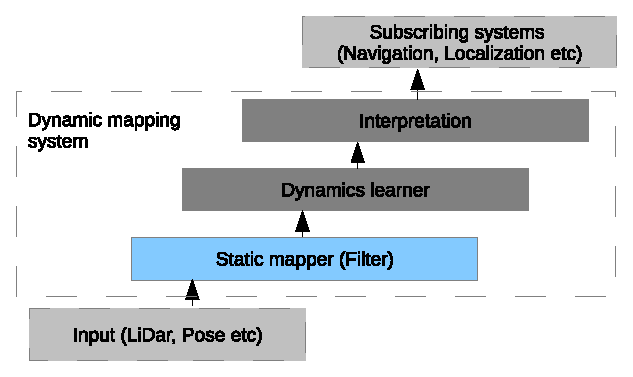
\includegraphics[scale=1]{chapters/static_mapping/figures/static_map_overview.eps}
		\caption{The static mapping in the dynamic mapping system}
		\label{fig:static_map_overview}
\end{figure}

In this chapter different sensor models are evaluated. Furthermore the effects of imperfect pose estimation is discussed and methods for incorporating various uncertainties are tested. 

%!TEX root = ../../report.tex
\section{Occupancy grid mapping}

An initial decision in mapping is how to represent the environment. A widely used method is the occupancy grid map, described in [REFERENCE, ELFE?]. It splits the environment into evenly sized cells. Each cell contains an occupancy value describing how occupied the cell is. Often 0 for completely free and 1 for completely occupied.  
Another widely used representation is the topological map \cite{topologyOrig}. Herein the environment is represented as position or landmark nodes connected by vertices in a graph structure. This representation was created for effective navigation in the environment. A drawback of the topological map is that it contains less metric information than the occupancy grid mapping \cite{mapbuildingSummary}.


Why occupancy grid ? (interface, recognised, used through put the community - considerations on other representation)

Mapping by inserting obstacle and free when observed.

Log odds

Real world test -> Results in bad maps.

Propagation of noise to avoid over confidence while still converging to the right solution. (Types of noise)


%!TEX root = ../../report.tex
\section{Laser Range Sensor Model}
\label{sec:laser_range_sensor}
When A. Elfes and H. Moravec introduced the occupancy grid map they also introduced the inverse sensor model used to update a map considering the uncertainties related to measurements \cite{elfesMoravecOccGrid}. 
A sensor characteristics is described with a forward sensor model, 
\begin{equation*}
	p(z_t|m_i,x_t)
\end{equation*}
which is the probability for measuring a distance given the location of the sensor and the obstacle the measurement hits. 
The inverse sensor model,
\begin{equation*}
	p(m_i|z_t,x_t)
\end{equation*}
converts these characteristics to describe the probability for occupancy of the map given the measurement. The last term in equation \vref{eq:occupancy_update} is the log-odds version of this value.
This principle is applicable for multiple sensors but in this project it is used for LIDARs. 


\subsection{Forward Sensor Model}
LIDARs are often modeled as multiple independent beams with four different types of noise models mixed together by a weighted average \cite{probRob}.
The areas under the noise models and the combined model is illustrated in figure \ref{fig:sensor_noise_model}.
\begin{figure}
\centering
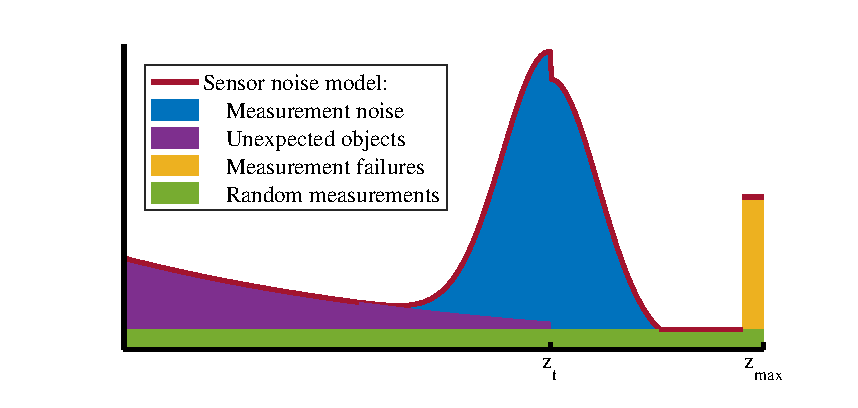
\includegraphics[scale=1]{figures/static_mapping/sensor_noise_model}
\caption{The beam sensor model for range finders is a mixture of noise models for different error types.}
\label{fig:sensor_noise_model}
\end{figure}


The small Gaussian measurement noise around the correct distance, arises from limited resolution of the sensor, atmospheric effects, etc. This noise is modeled as a normal distribution and should be taken into account when a sensor model is devised. 

The noise from unexpected obstacles stems from using a static map to represent a dynamic environment. When the robot senses the environment it will occasionally measure obstacles that are not present in the map, for instance moving people.

For LIDARs, failures can occur due to insufficient reflectance of light back to the sensor. 
These failures often cause a maximum range reading which are handled by removing measurements with maximum range.

The random measurements represents entirely random readings. These are modeled with a uniform distribution and should be taken into account in the sensor model.

S. Thrun proposed to learn occupancy grids from the forward sensor model with expectation-maximization \cite{probRob}.
This method reduces the effects of conflicting sensor model updates, causing incorrect addition or removal of obstacles. 
This demands for storing a batch of measurements and is computational expensive to perform. 
Therefore, it is more common to learn occupancy grids with an inverse sensor model where measurements are added incrementally according to equation \vref{eq:occupancy_update}. 

\subsection{Inverse Sensor Model}
The inverse sensor model describes the probability for a cell being occupied in an occupancy grid map given a sensor measurement and location. 
Many different inverse sensor models have been proposed to incorporate LIDAR measurements in a occupancy grid map. The individual rays are often assumed narrow and the orientation of it with respect to the robot is assumed ideal.
The simplest possible inverse sensor model is the 
ideal inverse sensor model. It assumes zero probability for occupancy before the measured distance, one at the measured distance, and $0.5$ after. The model shown in figure \vref{fig:sensor_model_std_dev01} is almost ideal.

\subsubsection{Elfes Sensor Model}
R. Merali and T. Barfoot \cite{sensorModelTuning} conducted a comparison and tuning of common inverse sensor models for laser rangefinders in a one dimensional simulated situation. It showed that the simple model with Gaussian noise proposed by A. Elfes in \cite{elfes} performed as good using only 2 parameters, as a 21 parameter approximation to the full Bayesian solution of the entire binary occupancy grid. They found that the model performed better, if the log-odds values were limited to -12.9047. This is also used in this work.

D. Joubert derives Elfes model in \cite{Joubert2014} by convolving a Gaussian function on an ideal sensor model. While this can be done analytically it is chosen to apply the yellow kernel shown in figure \vref{fig:sensor_model_std_dev01} to the ideal sensor model.
The distance to the obstacle is $0.275m$ and the standard deviation of the Gaussian kernel is $1cm$. 
SICK states the noise parameters for the S300 to be $\pm20mm$ systematic error and $\pm9mm$ statistical error, when measuring a distance of three meters \cite{lidarDatasheet}. 
Since the error might be subject variations and is used for ranges up to $30m$, the noise used in simulations for the MiR-100 is $1cm$ Gaussian noise. 
The maximum and minimal log-odds values are out of the scope, but they can be calculated from the probabilities with equation \vref{eq:occupancy_update}.


\begin{figure}[htbp]
	\centering
	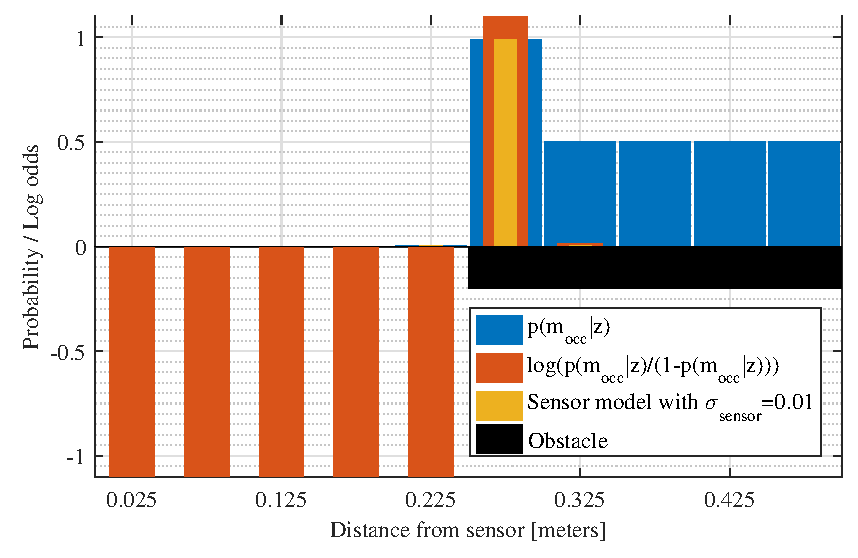
\includegraphics[scale=1.0]{figures/static_mapping/sensor_model_std_dev01}
	\caption{Elfes inverse sensor model with the used sensor's model.}
	\label{fig:sensor_model_std_dev01}
\end{figure}

Figure \vref{fig:sensor_model_std_dev025} shows an inverse sensor model with a standard deviation of $2.5cm$.
This indicates less trust in the measured distance. With this model more measurements are needed to reach as high an occupancy probability, as would be achieved with the ideal model. It can however be used to avoid overconfidence in measurements while still converging to the correct map if the measurement error is Gaussian distributed.

\begin{figure}[htbp]
	\centering
	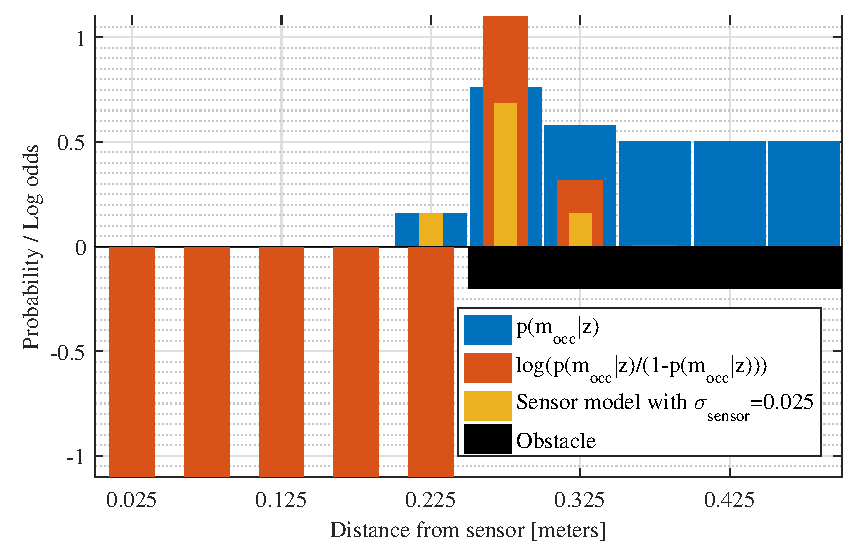
\includegraphics[scale=1.0]{figures/static_mapping/sensor_model_std_dev025}
	\caption{Elfes inverse sensor model with a larger standard deviation than that of the sensor's.}
	\label{fig:sensor_model_std_dev025}
\end{figure}

Even with the sensor noise modeled as shown in figure \ref{fig:sensor_model_std_dev01}, erroneous maps like the one shown in \ref{fig:elfes_ideal_with_poses} and \ref{fig:elfes_compare} are expected, due to localization errors.
The influence of the error could be diminished by incorporating the localization errors in the inverse sensor model.

\begin{figure}[htbp]
	\centering
	\begin{subfigure}[t]{0.45\textwidth}
		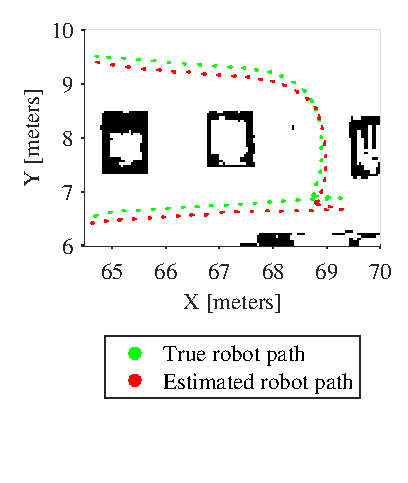
\includegraphics[scale=1.0]{figures/static_mapping/map_region_with_poses}
		\caption{Occupancy grid of the simulated world.}
		\label{fig:map_region_with_poses}
	\end{subfigure}
	\begin{subfigure}[t]{0.45\textwidth}
		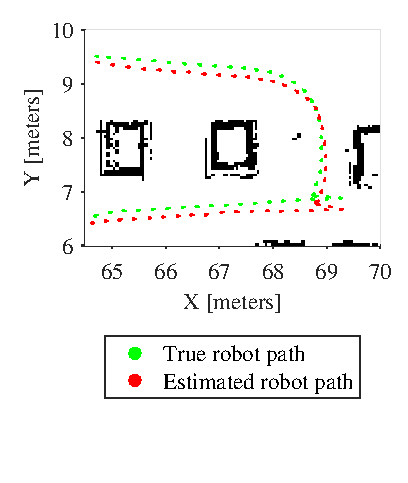
\includegraphics[scale=1.0]{figures/static_mapping/elfes_ideal_with_poses_no_decay}
		\caption{Mapped occupancy grid using the sensor model in figure \vref{fig:sensor_model_std_dev01}.}
		\label{fig:elfes_ideal_with_poses}
	\end{subfigure}
	\caption{Mapping results gained by simulating a MiR-100 robot with imprecise location.}
	\label{fig:simulated_location_error}
\end{figure}

\begin{figure}[htbp]
	\centering
	
\includegraphics[width=0.5\linewidth]{figures/static_mapping/elfes_ideal_no_decay}
	\caption{Comparison between the obstacles position in figure  \vref{fig:map_region_with_poses} shown in green and the mapped obstacles in figure \vref{fig:elfes_ideal_with_poses} shown in red. The overlapping yellow regions marks areas with successful mapping.}
	\label{fig:elfes_compare}
\end{figure}


%!TEX root = ../../report.tex
\section{Mapping with Location noise}
\label{sec:mapping_with_location_noise}

Traditional approaches to occupancy grid mapping assumes ideal localization \cite{probRob}. 
Hence the mapping amounts to updating the map with an inverse sensor model, like described in section \vref{sec:laser_range_sensor}.
This section investigates methods to improve mapping by incorporate localization noise.
While it is unrealistic to map the world exactly without knowing the robots exact pose, it is possible to adjust the sensor model based on the size of the estimated localization error.
By updating with larger regions with less values all the information is used, which leads to faster convergence to the correct map if the noise model is accurate.

\subsection{Monte Carlo localization}
The robot estimates its localization with an adaption of the ROS implementation \cite{ros_amcl} of the Adaptive Monte Carlo Localization(AMCL) \cite{Thrun200199}. It uses a particle filter to track the robot's pose in a known map. 

The estimated uncertainty on the localization is described with a covariance matrix. The covariance matrices for some of the locations the robot visited during navigation in an industrial environment is visualized as contour plots around the robots position(green) in figure \vref{fig:amcl_covariance}. 
The figure shows that the estimated standard deviation on the positional error generally is around $10cm$. Around the corner the estimated standard deviation however increase to more than twice that. This is reasonably since the map used by AMCL for scan matching was wrong in the top left corner of figure \vref{fig:amcl_covariance}. The estimated angular error also doubles when the robot reaches the corner.

In figure \vref{fig:simulated_small_world} the simulated world is shown. The corresponding map used by AMCL to estimate the robot pose is shown in \vref{fig:simulated_small_amcl_map}.

\begin{figure}[htbp]
	\centering
	\begin{subfigure}[t]{0.75\textwidth}
		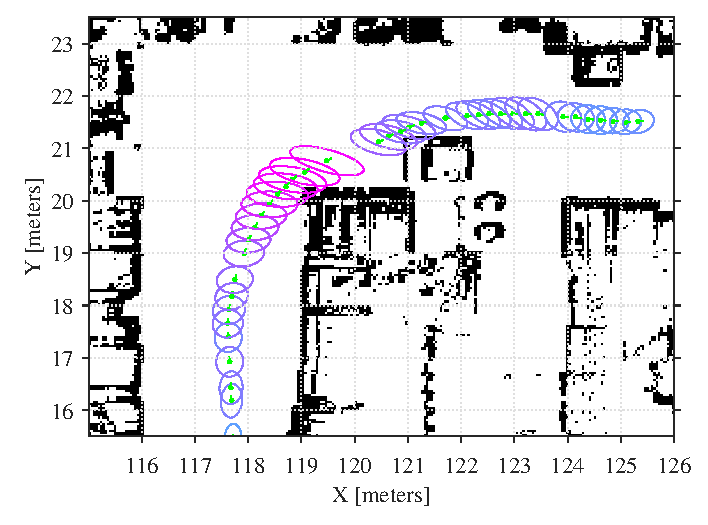
\includegraphics[scale=1.0]{figures/static_mapping/amcl_covariance}		
	\end{subfigure}
	\begin{subfigure}[t]{0.2\textwidth}
		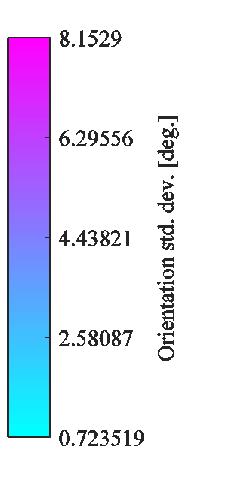
\includegraphics[scale=1.0]{figures/static_mapping/amcl_covariance_bar}
	\end{subfigure}
    \label{fig:amcl_covariance}
	\caption{Covariances estimated by AMCL in an industrial environment shown with contours marking one standard deviation around the robot's estimated pose(green).}
\end{figure}

It is clearly visible from the maps that AMCL was missing information about the world. The lack of correspondence between the maps causes the covariance of the pose estimate to increase.
Marked on figure \vref{fig:simulated_location_error} are the path the robot drove through the world, both the estimated and the true path.
A ROS bag was created of the run in order to ensure all methods was given the same input. 

\begin{figure}[htbp]
	\centering
	\begin{subfigure}[t]{0.45\textwidth}
		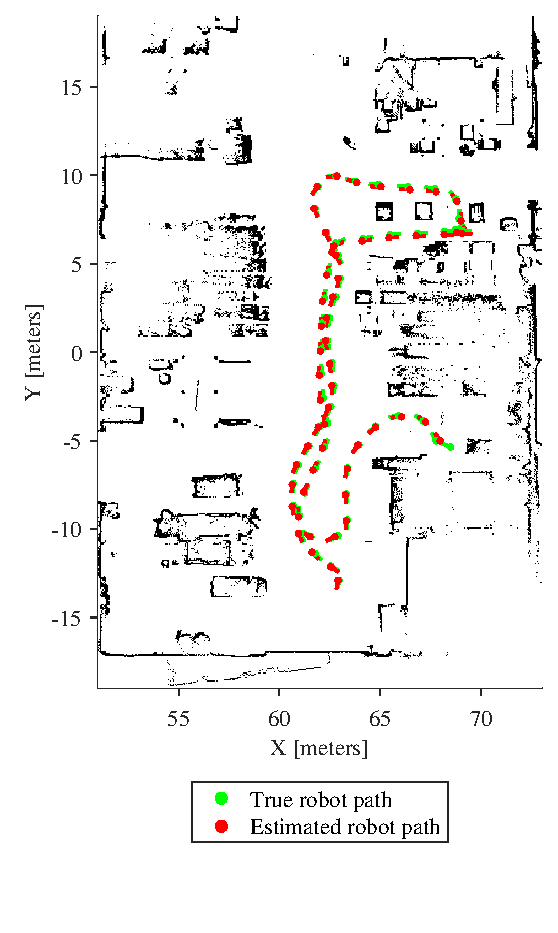
\includegraphics[width=\textwidth]{figures/static_mapping/simulation_poses_stage_map}
		\caption{World representation}
		\label{fig:simulated_small_world}
	\end{subfigure}
	\begin{subfigure}[t]{0.45\textwidth}
		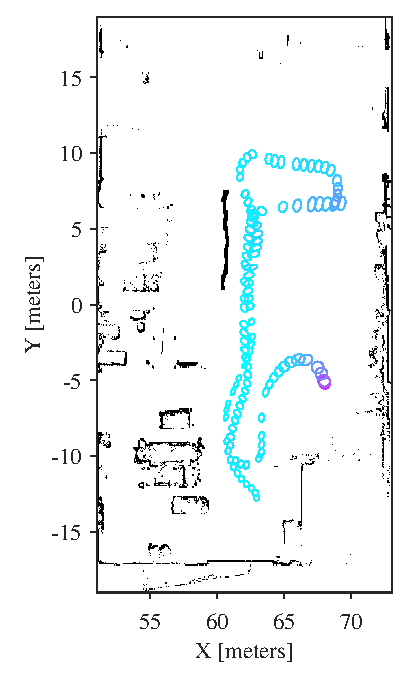
\includegraphics[width=\textwidth]{figures/static_mapping/simulation_poses_amcl_map}
		\caption{Map used by AMCL}
		\label{fig:simulated_small_amcl_map}
	\end{subfigure}
	\caption{Simulation of a MIR robot moving with imprecise location.}
	\label{fig:test_map_setup}
\end{figure}

\subsection{Reduced ideal Inverse Sensor Model}
\label{sec:reduced_ideal_sensor_model}
The ideal inverse sensor model can be modified to avoid over confidence in sensor measurements, when the localization is wrong by decreasing the update term. 
A version of this is shown in figure \vref{fig:reduced_ideal_sensor_model}, where the probability when observing free is $0.4$ and the probability at the measured distance($l$) is $0.6$. 

\begin{figure}[htbp]
	\centering
	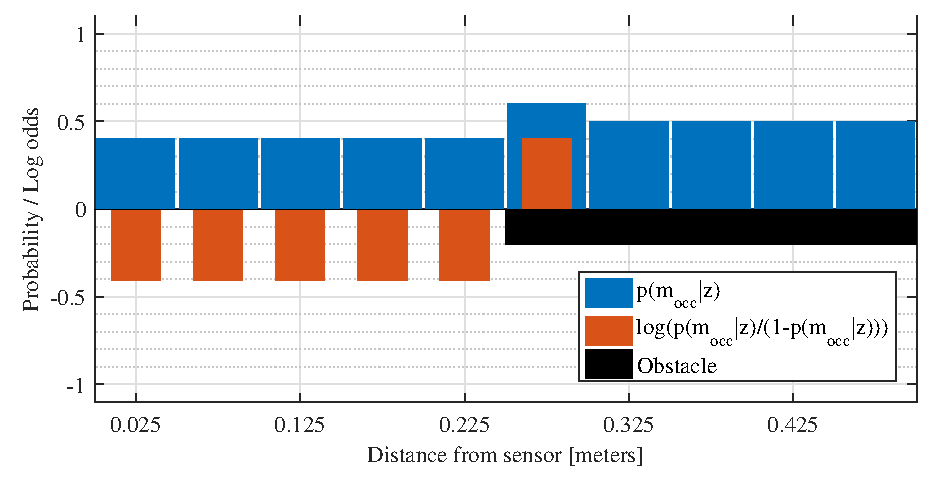
\includegraphics[scale=1]{figures/static_mapping/reduced_ideal_sensor_model}
	\caption{Reduced Ideal inverse sensor model}
	\label{fig:reduced_ideal_sensor_model}
\end{figure}

Despite the decrease in update values, the model can have tendency to be over confident in long measurements when the orientation is wrong.
This results in a removal of inserted obstacles when ray-traces wrongly go through them due to localization errors.
These effects are similar to the once shown in figure \ref{fig:particle_hector_sensor-croped}.
This is diminished by multiplying the log-odds values with equation \vref{eq:angle-weight}.

\begin{equation}
\label{eq:angle-weight}
weigth = 
\begin{cases}
1 - ( 2 \cdot \theta \cdot l ), & \text{if } 2 \cdot \theta \cdot l < 1\\
0, & \text{otherwise}
\end{cases}
\end{equation}

Where \(\theta \) is the standard deviation of the orientation estimate and \(l\) is the measured distance.

In order to account for the uncertainty of the position estimates another weight calculation, shown in \vref{eq:pose-weight}, is also tested.

\begin{equation}
\label{eq:pose-weight}
weigth = 
\begin{cases}
1 - ( 2 \cdot \theta \cdot l + 2 \cdot (\sigma_x + \sigma_y) ), & \text{if } 2 \cdot \theta \cdot l + 2 \cdot (\sigma_x + \sigma_y) < 1\\
0, & \text{otherwise}
\end{cases}
\end{equation}

Where \(\theta \) is the standard deviation of the orientation estimate, \(l\) is the measured distance, \(\sigma_x\) is the standard deviation of the position estimate in the x direction and \(\sigma_x\) is the equivalent in the y direction.
Both of the weight functions are also to be tested on the Elfes model.

\subsection{Monte Carlo Integration Inverse Sensor Model}
\label{sec:monte_carlo_sensor Model}
The monte carlo integration inverse sensor Model proposed by Joubert, Brink and Herbst \cite{Joubert2014},  uses the fact that particles used in Monte Carlo Localization with their likelihood weights(importance factors) approximates the robots uncertainty. 
It works by ray-tracing the sensor measurements with a weighted ordinary inverse sensor model from the particles' poses instead of the estimate d pose. 
Equation \vref{eq:monte_carlo_sensor_model} shows how a log-odds occupancy cell is updated with the right most term consisting of a weighted sum of inverse sensor models for $K$ particles.

\begin{equation}
log \frac{p(m_i|z_{1:t})}{1-p(m_i|z_{1:t})} = log \frac{p(m_i|z_{1:t-1})}{1-p(m_i|z_{1:t-1})} + \sum_{i=1}^{K} w_t^i log \frac{ p(m_i | z_t^i) }{ 1 - p(m_i | z_t^i) }
\label{eq:monte_carlo_sensor_model}
\end{equation}

It can be computational expensive to ray-trace the often several hundred measurements every tenth of a second from each of the often several hundreds of particles.
To avoid this, only the $K$ top most weighted particles can be used. 
This has the effect that the total sum of update values is reduced to the total sum of the weights for the used particles.
Depending on the spread of the distribution of the particles the amount of changes applied to the map per measurement varies.
Depending on processing capability and rate of measurements the number of used particles might be increased.

When using $30$ particles the map is updated with a sensor measurement on each of the two sensors as shown in figure \vref{eq:monte_carlo_sensor_model}.
The sensors' frames are shown around the robots base frame as green and red lines.
It is clear that it only updates the map weakly since the particles are far spread. 
The obstacles are updated at different positions since the particles are located at different positions. With the many particles this results in blurred lines, which has the highest value in the center.

The model uses a reduced ideal inverse sensor model similar to the one described in section \vref{sec:reduced_ideal_sensor_model}, where the probability for occupancy at the obstacle is $0.85$. The probability for free is set to $0.45$. 
It is chosen to optimize the reduced ideal inverse sensor model this way, since it is better at adding obstacles as shown in figure \vref{fig:particle_sensor}.

The reason to the methods tendency to remove obstacle is that small difference in orientation between the particles results in ray-traces going through the obstacles as shown in figure \vref{fig:particle_sensor}. The weight for each used particle has been normalized to making the rays clearly visible. 
The figure shows how most of the ray-traced inverse sensor models results in similar looking maps along the rays. 
It can be seen how the model have built a map where there are a small probability for occupancy along the rays with similar distance by rotated around the robot's pose (red square). 

\begin{figure}[htbp]
	\centering
	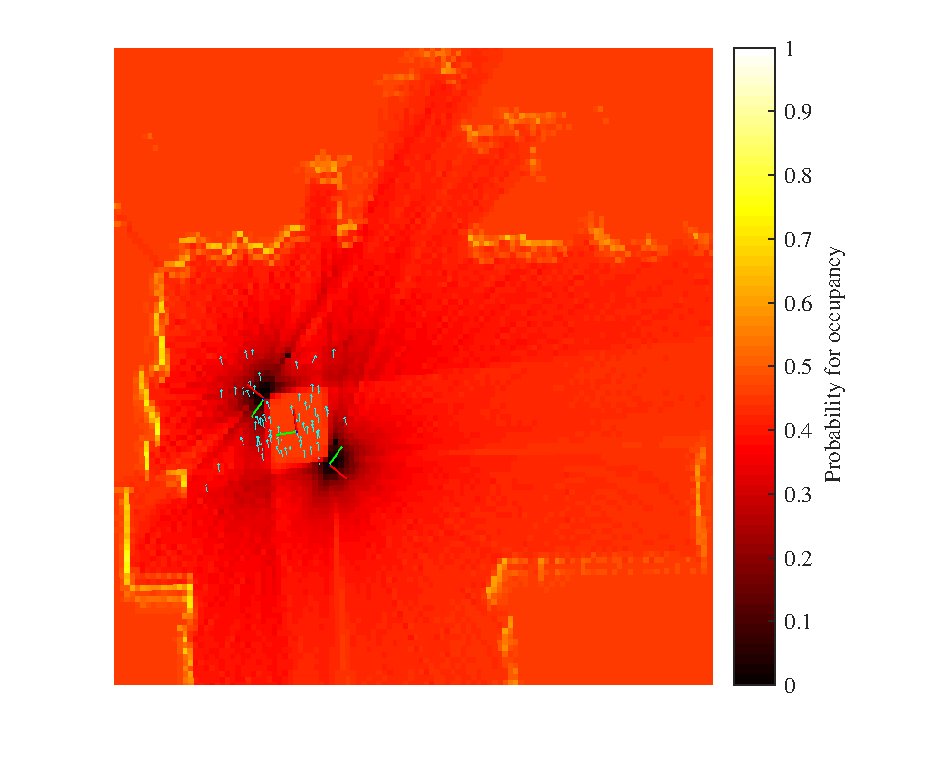
\includegraphics[scale=1.0]{figures/static_mapping/particle_principle}
	\caption{Map after ray-tracing with a modified reduced ideal inverse sensor model from all particles.}
	\label{fig:particle_principle}
\end{figure}

\begin{figure}[htbp]
	\centering
	\begin{subfigure}[t]{0.45\textwidth}
		
\includegraphics[width=\textwidth]{figures/static_mapping/monte_carlo_map_hector}
		\label{fig:particle_hector_sensor-croped}
		\caption{Monte Carlo integration using Elfes inverse sensor model shown in figure \ref{fig:sensor_model_std_dev01}.}
	\end{subfigure}
	\begin{subfigure}[t]{0.45\textwidth}
		
\includegraphics[width=\textwidth]{figures/static_mapping/monte_carlo_map_optimized}		
		\label{fig:particle_shot-croped}
		\caption{Optimized inverse sensor model}
	\end{subfigure}
	\caption{Mapping in simulation using Monte Carlo integration inverse sensor Model with different sensor models for ray-traycing.}
\end{figure}

\begin{figure}[htbp]
	\centering
	
\includegraphics[width=0.7\linewidth]{figures/static_mapping/particle_sensor}
	\caption{Example map with few LIDAR measurements from the five highest weighted particles.}
	\label{fig:particle_sensor}
\end{figure}

\subsection{Cone based model}
An attempt to represent the pose uncertainty in the static mapping is a model based on a sonar-like cone. 
The idea is to represent the uncertainty in the localization of the robot on the inverse sensor model by representing it with the model in figure \vref{fig:cone_with_noise_top}.  
This cone consist of the center area, the left side cone and right side cone. 
As the model is based on a sonar cone model \cite{probRob}, the values of a cell is determined by the distance from the origin and the angle to the straight line to the target. The changes from the original sonar model is the center section which splits the two cone halves. 

The angle \(\theta\) is equal to the standard deviation of the orientation estimate. 
The width of the center area, w, is determined by the sum of the projection of the standard deviation in the x and y directions perpendicular to the ray direction. 

The value of a cell is determined by the distance from the origin line. 
The value at the point $p$ in figure \vref{fig:cone_with_noise_top} is determined by the the distance l.
The width, m, of the marking cone is determined by the position error projected onto the ray.

It is possible to add a weight to cell value. This weight is given by equation \vref{eq:cone-weight}.
\begin{equation}
\label{eq:cone-weight}
weigth = 
\begin{cases}
1 - ( 2 \cdot \theta \cdot l + w), & \text{if } 2 \cdot \theta \cdot l + w < 1\\
0, & \text{otherwise}
\end{cases}
\end{equation}

\begin{figure}[htbp]
	\centering
	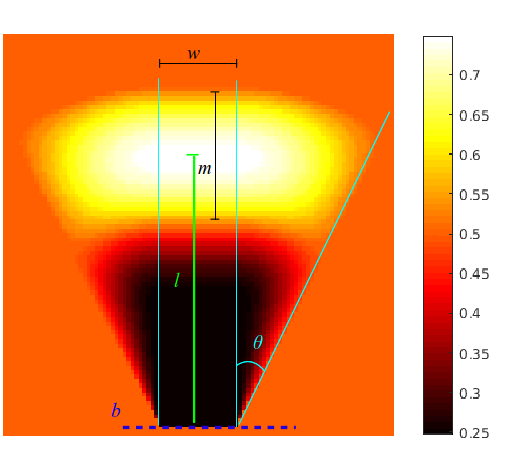
\includegraphics[width=\textwidth]{figures/static_mapping/cone_noise_top}
	\caption{Cone representing pose noise}
	\label{fig:cone_with_noise_top}
\end{figure}

\subsection{Comparison of Inverse Sensor Models}
In order to compare the various mapping methods a metric, for determining the accuracy of a map, is needed. One of the methods for comparing to occupancy maps is the Map Score, first proposed in \cite{MoravecMartin}. The score is calculated as the squared error between the occupancy for each cell in two maps, as seen in equation \vref{eq:MapScore}.

\begin{equation}
\label{eq:MapScore}
Score = \sum_{n=0}^{N} (m_{n} - o_{n})^2
\end{equation}

N is all cells in the maps m and o. 
This gives a simple result that indicates how alike two maps are. 
However, as most maps contains vastly more free space than occupied space this might skew the result. 
A map can receive a higher score for asserting strong statements about free cells but not mapping obstacles very accurate. 
As the obstacles are vital parts of the map this is not desired. 
To overcome this it is suggested to only use cells where either one of the maps have an occupied probability higher than \(0.5\) \cite{Sullivan2003}, this will be denoted Sum of Squared Error (SSE).
As the SSE does not distinguish between the number of cells touched it can be useful to normalize the score with the number of cells in the map tested. This will be denoted the Mean Squared Error (MSE).  

\subsubsection{Results}
The methods was tested on a ROS-bag of a path through a simulated environment. 
The localization of the robot was not perfect due to differences between the world representation and the one used by AMCL.
The world map and the robots representation can be seen in figure \vref{fig:test_map_setup}.
As the world map has obstacle cells completely surrounded by other obstacle cells and therefore impossible for the robot to see the world map was adjusted before the comparison. Only obstacle cells with at least one neighboring free cell is to be considered. Obstacle cells with no free cell neighbors are set to unknown. 

In figure \vref{fig:comparison_obstacle_error} the results for each method is shown. The SSE in calculated as equation \vref{eq:MapScore}, but only for cells where either the ground truth, or the test map is above the unknown value on $0.5$, and the ground truth value is different from this value. As the SSE represent the error between the true and the estimated map, a lower result is advantageous. In this test, the reduced ideal model with uncertainty decay received the lowest score. Both Elfes and the reduced ideal models perform better when angle decay is used. This suggests using the uncertainty of orientation estimate is preferable. Similarly when position uncertainty is added they perform even better. Of the two methods that incorporates both uncertainty for the orientation and position estimate directly in the methods, the Monte Carlo performs best, but no where near as good as the Reduced Model with pose decay. 
 
Things change, however, when observing the results based on the MSE of figure \vref{fig:comparison_obstacle_error_per_cell}. 
This score is calculated as the scores of figure \vref{fig:comparison_obstacle_error} divided by the number of cells with occupancy probability greater than \(0.5\), in either the test maps or the ground truth, thus representing a mean error per obstacle cell.
Using the MSE the Monte Carlo method outperforms the other methods, having a result of \(\approx 0.38\), with the closes contestant, the Reduced Ideal model with decay, at \(\approx 0.47\).\\

\begin{figure}[htbp]
	\centering
	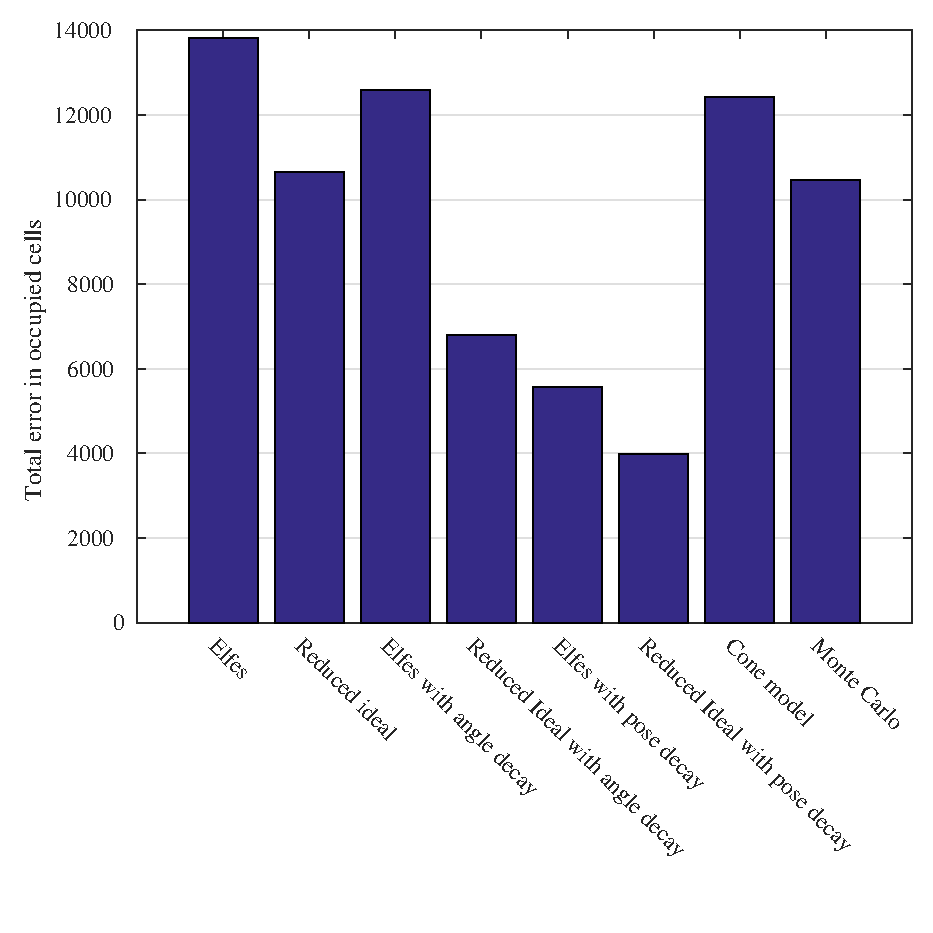
\includegraphics[scale=1]{figures/static_mapping/comparison_obstacle_error}
	\caption{Sum of Squared Error - obstacles only}
	\label{fig:comparison_obstacle_error}
\end{figure}

\begin{figure}[htbp]
	\centering
	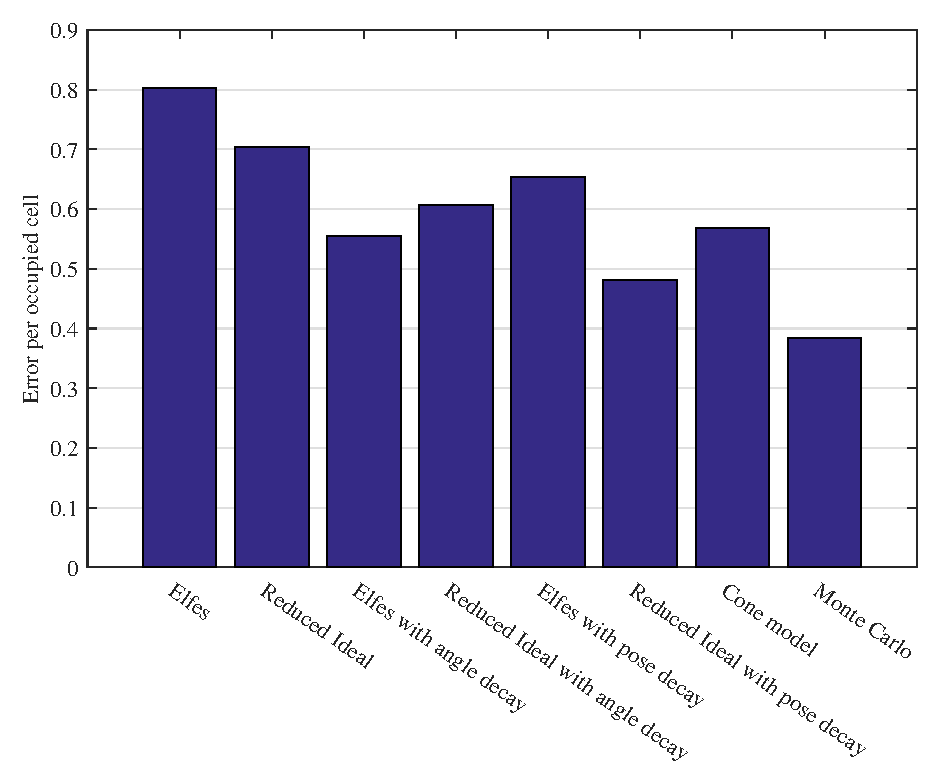
\includegraphics[scale=1]{figures/static_mapping/comparison_obstacle_error_per_cell}
	\caption{Mean Squared Error}
	\label{fig:comparison_obstacle_error_per_cell}
\end{figure}

The top scorers in both scoring systems are the Monte Carlo and the Reduced Ideal model with pose decay. As each of the two methods where at the top in one of the scoring methods, determining the best is not straight forward.

In order to further investigate the differences between the two methods the generated maps are to be compared and contrasted to the ground truth map. 
Figure \vref{fig:box_region_comparison} show a comparison, of a region, between the methods against the ground truth.
The Monte Carlo method produces larger occupied areas, due to the pose uncertainty. The occupied areas are a blur around the edges of the true obstacles. 
Comparing this to the Reduce Ideal method, which has marked sharper edges. 
These edges, however, are not perfectly located on the outer edge of the obstacles. 
This problem stems from a consistent pose error that is not perfectly handled by the pose decay. 

\begin{figure}[htbp]
	\centering
	\begin{subfigure}[t]{0.45\textwidth}
		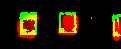
\includegraphics[scale=1.5]{figures/static_mapping/color_diff_monte_carlo}		
		\label{fig:monte_carlo_mapsec1}
		\caption{Monte Carlo method}
	\end{subfigure}
	~ %add desired spacing between images, e. g. ~, \quad, \qquad, \hfill etc. 
	%(or a blank line to force the subfigure onto a new line)
	\begin{subfigure}[t]{0.45\textwidth}
		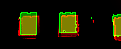
\includegraphics[scale=1.5]{figures/static_mapping/color_diff_ideal_decay}
		\label{fig:ideal_deacy_mapsec1}
		\caption{Reduced Ideal with decay}
	\end{subfigure}
	\caption{Region of the generated maps and the ground truth. The ground truth occupancy is represented in green and the generated maps' occupancy in red. Following from that overlaps trend to yellow.}
	\label{fig:box_region_comparison}
\end{figure}

In the further development of the mapping in dynamic environment it is chosen to use the Reduced Ideal model with pose decay. This method is considered most suitable for the task due to its ability to suppress pose uncertainties while still maintaining a fairly accurate representation of the environment. 

%!TEX root = ../../report.tex
\section{Mapping an Industrial Environment}
\label{sec:mapping_at_scan}
The reduced ideal inverse sensor model superior performance to map static obstacles have been verified by navigating a MiR-100 through the production line at SCAN A/S 19 times.
Figure \ref{fig:scan_overview_drawing} shows a part of the production area and the map that was created with the robots native Hector SLAM algorithm just before conducting the experiment.
The map is visualized with additive RGB colors where obstacles on the SLAM map is pure red. 
The map created with the reduced ideal model and the Elfes model shown in figure \ref{fig:sensor_model_std_dev01} is green and blue respectively.
The amount of color added is proportional to the estimated occupancy probability with none being certainly free and saturated meaning certain occupancy. 
The green and blue colors indicates obstacles that was not present when mapping or wrongly positioned obstacles.
The green area in the lower left part of the map shows obstacles that was not present when mapping, and the green area within the pallets to the right marks wrong estimates of occupancy.

\begin{figure}
    \centering
    \includegraphics[width=1\linewidth]{chapters/evaluation/figures/scan_overview_drawing}
    \caption{Mapping results of a region of the SCAN environment, shown with additive RGB color encoding. Red is the SLAM'ed map, green is the OG made with the reduced ideal model and the red is the OG made with Elfes model.}
    \label{fig:scan_overview_drawing}
\end{figure}

The lack of blue influence on the edges of the pallets is most likely due to the Elfes inverse sensor model's very large clearing update values without consideration for localization errors.
The fact that the wall in the lower right corner is partly white, and are hence mapped by all the methods, indicates that it is especially the lack to account for the errors in the estimated orientation that causes the problems. 
The problem is similar to the one experienced with the Monte Carlo integration method described in section \ref{sec:monte_carlo_sensor Model}.
On these walls there is no free area behind so smaller errors in angle will not result in a clearing of obstacles due to long ray-traces with wrong direction.

The domination of yellow on the edges of the pallets facing towards the corridor where the robot navigated, indicates that the proposed integration of localization noise in the inverse sensor model is appropriate for mapping. 
%!TEX root = ../../report.tex
\section{Summary}
In this chapter various methods of including pose estimation noise into an occupancy grid mapping approach has been evaluated. 
The method that was chosen is the reduced ideal model with pose decay because of its ability to avoid overconfidence in observations made under error-prone localization. 
The occupancy probabilities chosen for free is \(0.4\) and \(0.6\) for occupied. The pose estimation noise is incorporated as a weight that reduces the certainty as the estimation variance increases.  

These elements has been inserted in the static mapper block, as seen in figure \ref{fig:static_map_detail}. 
The sensor input and pose estimation is combined and inserted in the static map as determined by the sensor model and noise weight.
Based on the estimated pose and observed LIDAR scans a static occupancy grid map is created with the sensor model. 
At fixed intervals the static map is then provided as a snapshot to the dynamic learner and then cleared. 

\begin{figure}[htbp]
	\centering
	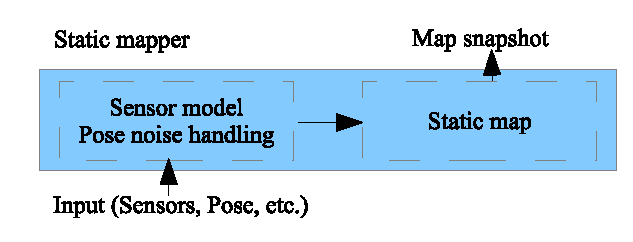
\includegraphics[scale=1]{chapters/static_mapping/figures/static_map_detail.eps}
	\caption{Static mapping module concept}
	\label{fig:static_map_detail}
\end{figure}


%!TEX root = ../../report.tex
\chapter{Mapping of Dynamic Areas}
\label{mapping_of_dynamic_areas}
This chapter investigates possible methods for learning the dynamic properties of an area in order to improve localization and navigation.
Specifically the following aim is considered:

\begin{enumerate}
    \setcounter{enumi}{1}
    \item Long-term, fast, adaptive map representation of dynamic environments
\end{enumerate}

The dynamic learner module is shown in figure \ref{fig:dynamic_learner_overview} in relation to the rest of the dynamic mapping system. It receives the static maps and uses these as the basis for learning the dynamics.  

\begin{figure}[htbp]
	\centering
	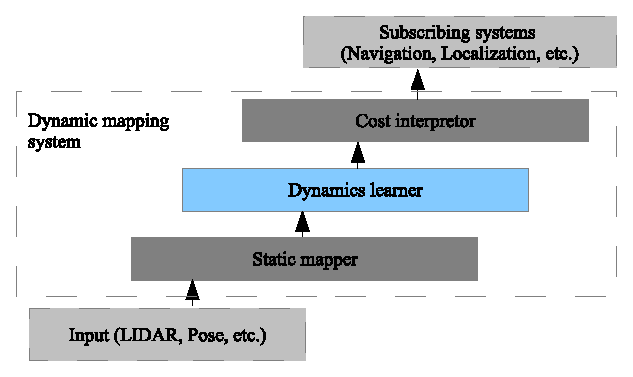
\includegraphics[scale=1]{chapters/mapping_of_dynamic_areas/figures/dynamic_overview.eps}
	\caption{The static mapping in the dynamic mapping system}
	\label{fig:dynamic_learner_overview}
\end{figure}

\section{Learning Dynamics of Occupancy Grid}
\label{sec:learning_dynamics_of_env}

\subsection{Previous work}
Learning the dynamics of an environment is a subject with ongoing research.
An early system for mapping the dynamics of the environment in a occupancy grid was the Temporal Occupancy Grid (TOG) proposed by Arbucle et al. \cite{Arbuckle2002}. The TOG system maintains several occupancy grids based on different time scales. This requires storing the observations for the time the longest TOG spans. It can be difficult to determine the time scales needed to estimate the differently and changing dynamic behaviors in the environment.

Biber and Duckett \cite{Biber2005} proposes a method for mapping environment dynamics with maps that represent observations taking over different periods of time. The method is here denoted as Temporal Sample Map (TSM). The maps are updated by incorporating measurements using different recency weighted running average functions. These functions are estimated by removing random observations. The highly dynamic obstacles are considered as outliers and up to $50\%$ of them are removed by using the median measurement.

An avenue of thought that has received quite a lot of attention is the representation and learning of a Markov process based grid. A Markov Chain based grid was introduced by Sarinnen et al. \cite{Saarinen2012} called Independent Markov Chain Occupancy grid map (IMAC). This method represents each cell as a Markov process that can be in either of the states; free or occupied. 

\begin{figure}[tbph]
	\centering
	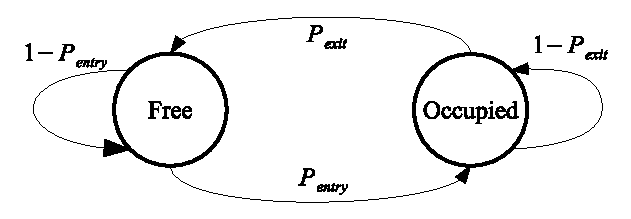
\includegraphics[width=0.7\linewidth]{chapters/mapping_of_dynamic_areas/figures/markow_occupancy_model}
	\caption{Markow chain for occupancy states borrowed from \cite{Saarinen2012}}
	\label{fig:markow_occupancy_model}
\end{figure}

The transitions is modeled as Poisson processes and the rate parameters is estimated as Gamma distributions. This gives in total four variables for each cell, which are used to interpret the type of dynamic for the cell. 

Another method for learning the map dynamics using Hidden Markov Models (HMM) is described by Meyer-Delius et al. \cite{Meyer-Delius2012}. This method uses the same possible states as the IMAC, but as it is a HMM the states are not directly observable thus it is possible to incorporate sensor uncertainty. In order to learn the parameters of the model two methods are used; an offline and an online approach. The offline approach requires storing all observations and then iteratively learn the parameters using the expectation-maximization algorithm. The online version of the parameter learning algorithm, developed by Mongillo and Deneve \cite{Mongillo2008} eliminates the need for storing the whole observation set. Instead only 16 values has to be stored for each cell and the iterative learning can be done online. The online method is capable of handling changing dynamics by using a forget factor. 

A different approach to mapping the dynamics is the Frequency Map Enhancement (FREMEN) proposed by Krajník et al. \cite{Krajnik2014}. This method models the dynamics of each cell by its primary frequency components. 
For prediction of future state the frequencies are reconstructed to a signal, which determines the predicted cell value. 
These uses a limited and constant number of parameters per cell. However, the method also requires the storage of time spans where the prediction went wrong in order to determine when a new model is needed. This significantly increases the memory requirements of the method.

With the reconstructed signal it is possible to predict infinitely long out in the future if it object moves with that frequency. 
This is not the case for Markow processes where the predicted probability for being in a state stabilizes on a constant, after many state changes.
There are also disadvantages with the method.
The most prominent comes from the fact, that it is impossible to recover a signal with a frequency lower than the Rayleigh-frequency of $1/T$, where $T$ is the period. 
This demands for storing measurements for the time period in which objects appears, disappears and appears again. This period can everything from hours for vehicles to days or weeks for stocked product parts. 
It might be possible to degrease the amount of stored information by only storing the average taken over periods, but then it is impossible reconstruct objects moving faster than the period which the average is taken. 

The characteristics of the six methods to improve occupancy grid mapping by learning the dynamics of the environment are outlined in table \ref{tab:learners_characteristics}.

\begin{table}[htbp]
    \centering
    \caption{Characteristics of methods to learn dynamics in occupancy grids.}
    \label{tab:learners_characteristics}
    \begin{tabular}{p{2.6cm} | p{1.6cm} | p{4.cm} | p{2.6cm} | p{1.6cm}}
        \toprule
        \textbf{Name} & \textbf{Memory} & \textbf{Dynamic representation} & \textbf{Learning method} & \textbf{Handles dynamics} \\
        \rowcolor[gray]{0.925}
        TOG & High & Time averaged OG & Online batch & Yes \\
        TSM & High & Time  averaged OG & Random sample replacement  & Yes\\
        \rowcolor[gray]{0.925}
        IMAC & Low & Markov parameters & Online iterative & Yes \\
        HMM - Offline & High & Markov parameters & Offline batch  & No \\
        \rowcolor[gray]{0.925} 
        HMM - Online & Low & Markov parameters & Online iterative & Yes \\
        FREMEN & Medium & Frequency components & Online batch & Yes\\
        \bottomrule
    \end{tabular}
\end{table}

\subsection{Methods ability to learn Markow Processes}
The described methods that models dynamic with Markow processes are compared with a simple simulation where a grid cell are occupied by a dynamic obstacle. 
Whether the cell is occupied or free is controlled by a Markow process with $0.9$ probability for entering and $0.2$ probability for exiting the cell. 
The process is observed by an one dimensional range sensor, which can measure too short with a probability of $0.16$, in which case the online-HMM are propagated one step without adding new information and the IMAC is left unchanged.
There is an equal probability for the sensor measuring a range too far, which results in a reading of an empty cell independently of the cell's state. 
Figure \ref{fig:markow_learning} shows that IMAC is unable to converge to the correct state transition probabilities, where as the HMM-online method that incorporate the uncertainties in measurements slowly converges toward them.
The state transitions estimated by IMAC are so far from the actual parameters that they are almost useless for prediction. 
The number of measurements needed for HMM-online to converge is however very large.
Considering that the simulation is setup so that the object has a considerable possibility of moving between each measurement, it will be very time consuming to learn the transition probabilities for obstacles moving at days between.

\begin{figure}[htbp]
    \centering
    \begin{subfigure}[t]{0.45\textwidth}
        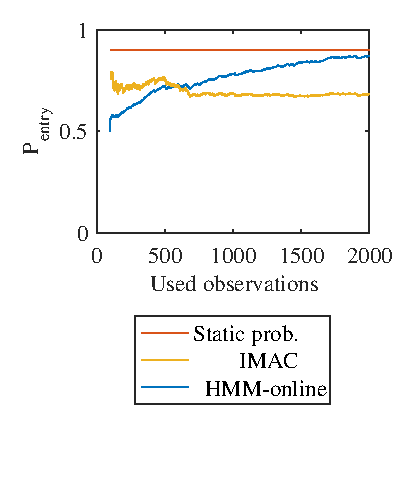
\includegraphics[width=1.0\textwidth]{chapters/mapping_of_dynamic_areas/figures/markow_learn_1d_entry}	
        %\caption{}
        %\label{fig:markow_learn_1d_entry}
    \end{subfigure}
    \begin{subfigure}[t]{0.45\textwidth}
        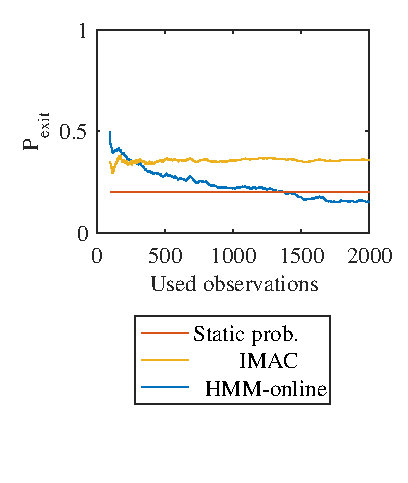
\includegraphics[width=1.0\textwidth]{chapters/mapping_of_dynamic_areas/figures/markow_learn_1d_exit}
        %\caption{}
        %\label{fig:markow_learn_1d_exit}
    \end{subfigure}
    \caption{Learned state transition probabilities compared to the simulated Markow process.}
    \label{fig:markow_learning}
\end{figure}

\section{FreMEn - Predicting future occupancy}
\label{sec:fremen}
The  Frequency Map Enhancement (FreMEn) method models the dynamics of each cell by its primary frequency components. It has successfully been applied to improve mobile robots ability to perform feature-based localization \cite{online_fremen} and topological navigation \cite{fentanes2015}. Here Krajník et al. argues for approximating the appearance and disappearance of obstacles with multiple periodic sinus signals, since people often moves them as part of daily routines. As discussed in section \ref{sec:characteristics_in_industrial_environments} this might also be the case in the industrial environments in focus here. Resent work in \cite{life_long_exploration}, shows how the often violated assumption in FFT about a fixed sampling rate is met by incrementally adding sparse and irregular observations. Where the approach usually uses the number of frequency components(m) that minimizes the difference between predicted states and measurements, it is chosen to use the typical order m=2 \cite{life_long_exploration} for all cells. This will probably decrease the prediction performance, but enables online updates without having to store observations for evaluation.

The online variant of the approach updates the parameters shown in equation \ref{eq:fremen_time} for each new measurement $s(t)$. 
The average occupancy probability $\alpha_0$ models the $0Hz$ signal and is updated with a new measurement online. 
The number of measurements n is incremented. There is one of the complex numbers $\gamma_k$ and $\beta_k$ for each $\omega_k=1/T_k$ . 
$T$ is calculated with equation \ref{eq:fremen_update} for each frequency, where N is the 20 used frequency components and epsilon is the smallest period time, which is one minute here. 
The values of consecutive $T_k$ is close for large values of $k$, which is advantageous if most of the obstacles moves with a period close to $\epsilon$.

\begin{equation}
    T_k = \frac{N \epsilon}{k+1}
    \label{eq:fremen_time}
\end{equation}

The real and imaginary part of $\gamma_k$ and $\beta_k$ are updated as the running average. $\gamma_k$ is the part of the signal with the frequency $2 \pi \omega_k$ and $\beta_k$ is the part of this signal which are modeled by the $0Hz$ component of the signal.

\begin{eqnarray}
&\alpha_0 = \frac{1}{n+1}(n \alpha_0 + s(t)) \nonumber \\ 
&\gamma_k = \frac{1}{n+1}(n \gamma_k + s(t) e^{-j \omega_k t}) \forall \omega_k \in \Omega  \\
&\beta = \frac{1}{n+1}(n \beta_k + \alpha_0 e^{-j \omega_k t}) \forall \omega_k \in \Omega \nonumber \\
&n = n + 1 \nonumber
\label{eq:fremen_update}
\end{eqnarray}

When predicting the state of a cell at time $t$ the signal components are calculated with equation \ref{eq:fremen_freq_component}.

\begin{equation}
    \alpha_k = \gamma_k - \beta_k \forall \omega_k \in \Omega
    \label{eq:fremen_freq_component}
\end{equation}

Then $ \Omega $ is ordered based on $ | \alpha_k | $ to enable calculation of equation \ref{eq:fremen_predict} using only the $m$ most prominent frequency components. As previously described, we use two frequency components ($ m=2 $) for each cell.

\begin{equation}
p(t) = \zeta \left( \alpha_0 \sum_{k=1}^{m} |\alpha_k| cos(\omega_k t + arg(\alpha_k))  \right)
\label{eq:fremen_predict}
\end{equation}

The function $\zeta$ clamps the expected probability to a value between zero and one. The $arg$-function returns the angle of the complex number with respect to the x-axis.
The occupancy state at time $t$ is predicted as occupied if $p(t)$ is above $0.5$ and as free otherwise.

\begin{figure}[htbp]
\centering
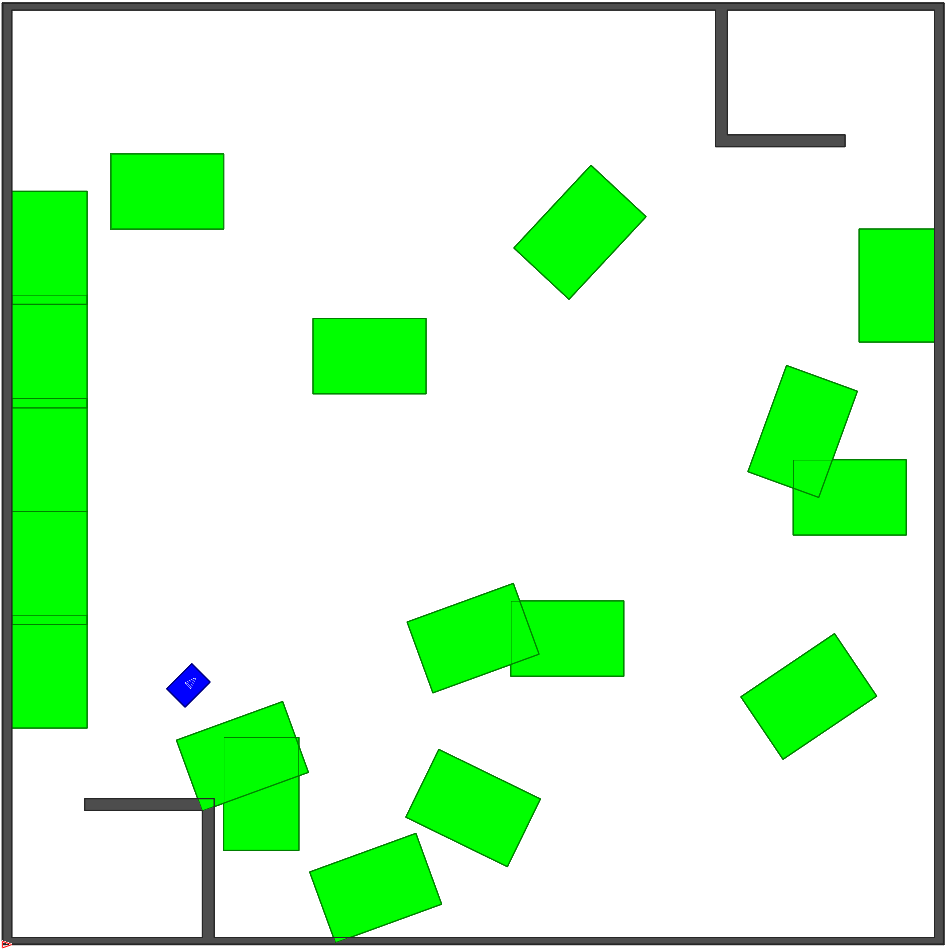
\includegraphics[width=0.4\linewidth]{chapters/mapping_of_dynamic_areas/figures/simulated_environment}
\caption{Screen shot of Stage simulator showing a MIR 100 robot navigating around obstacles which appears and disappears at fixed intervals.}
\label{fig:simulated_environment}
\end{figure}

The methods ability to predict future occupancy states are evaluated in a Stage simulation where many boxes moves in and out at various and fixed, intervals. 
The robot continuously navigates from the lower left corner that are partly surrounded by walls to the top right corner, while the red and green boxes moves around.
The measurements from the simulated LIDAR are incorporated in a temporary local map using the reduced ideal inverse sensor model update method described in section \ref{sec:reduced_ideal_sensor_model}. 
The update values for the sensor model is reduced to incorporate uncertainties in localization.
For every fifth second a global map of FreMEn cells are updated with \ref{eq:fremen_update} where $s(t)$ is the probability for occupancy in the local map. 
The local map is then cleared and the process continues.

\begin{figure}[htbp]
    \centering
    \begin{subfigure}[t]{0.49\textwidth}
        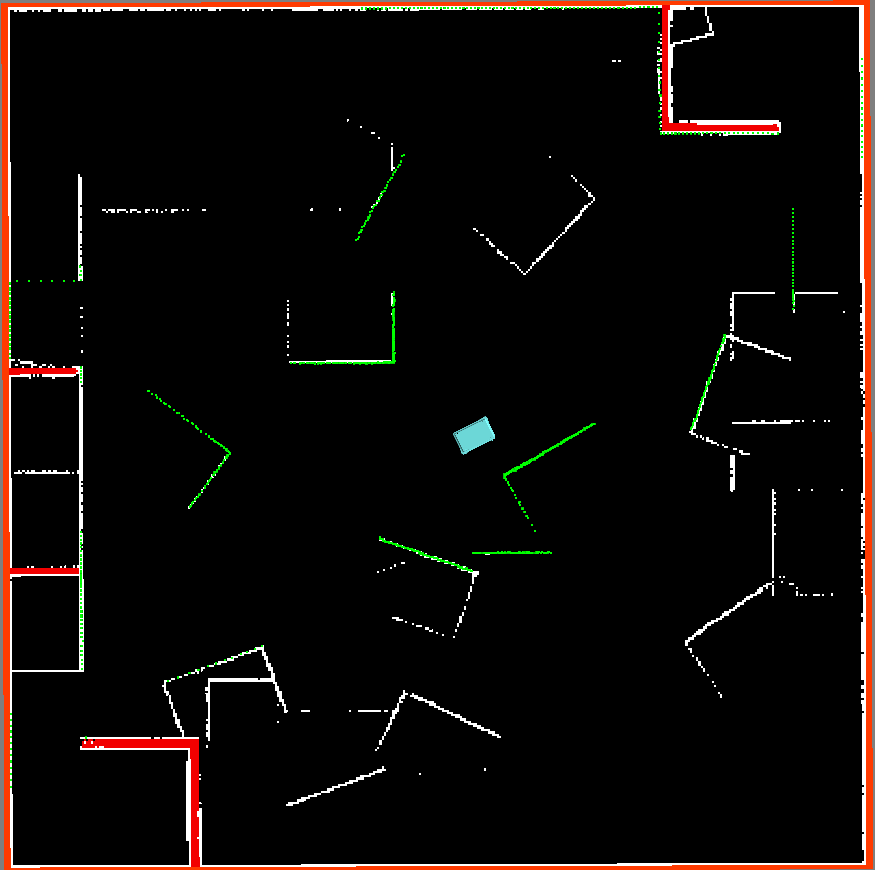
\includegraphics[width=1.0\textwidth]{chapters/mapping_of_dynamic_areas/figures/fremen_ideal_simulation}	
        \caption{Predicted map without noise.}
        \label{fig:fremen_ideal_sim}
    \end{subfigure}
    \begin{subfigure}[t]{0.49\textwidth}
        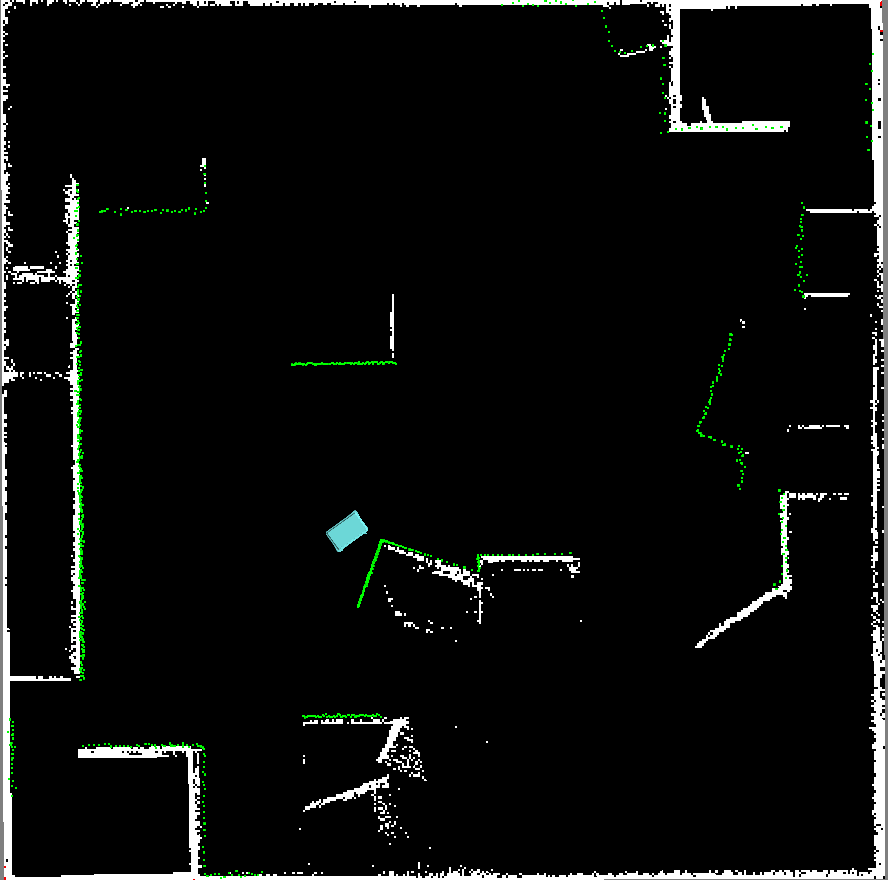
\includegraphics[width=1.0\textwidth]{chapters/mapping_of_dynamic_areas/figures/fremen_with_decay_last}
        \caption{Predicted map with realistic sensor and localization noise.}
        \label{fig:fremen_sim_with_noise}
    \end{subfigure}
    \caption{Robot navigating in the map predicted with FreMEn where the the green dots marks ends of LIDAR readings.}
\end{figure}

To evaluate the predictive strength of FreMEn it is used to predict the appearance of obstacles each time a new measurement is added from the local map. 
Figure \ref{fig:fremen_ideal_sim} shows how FreMEn correctly predicts the appearance of many of the obstacles when the robots exact position is used to incorporate exact LIDAR measurements. 
Figure \ref{fig:fremen_avg_miss_with_noise} shows a more realistic simulation with Gaussian noise on LIDAR measurements with a standard deviation of one centimeter and localization using AMCL with a static map representation.
Here some of the obstacles are predicted to have moved while they in fact are still present, as shown in the middle to the right in figure \ref{fig:fremen_avg_miss_with_noise}.

FreMEn's lack of ability to predict future measured obstacles is also apparent in the average correctly predicted observations of obstacles. This measure is calculated with equation \ref{eq:average_predict_score}, where $s$ is the state that can be occupied, or free, and $n_cells$ is the number of cells that are either observed or predicted as occupied.

\begin{equation}
    \text{Average correct obstacle prediction} = \left[1- \frac{\sum\limits_{i=1}^{n_{cells}} \left\|s_{predict}(i)-s_{observation}(i)\right\|}{n_{cells}}
    \right]\cdot 100
    \label{eq:average_predict_score}
\end{equation} 

This is shown in figure \ref{fig:fremen_avg_correct_predictions} where the good prediction percent on $74.0\%$ drops to $46.9\%$ with the addition of noise.
From the experiment without noise it is concluded that the learned periodic appearance of obstacles in a grid with FreMEn is useful for predictions.
In the presence of noise the signals within the cells becomes more complicated, and the measurements used for comparison is not always correct.
This, combined with the fact that obstacles placed by humans probably will not move in and out of grid cells so consistently as in this simulation, leads us to believe that the implemented method is not useful for online update of the occupancy grid map used by AMCL.
It might however be possible to alter the method, or combine it with others, to take advantage of the methods ability to predict presence of obstacles many hours after the last observation.
The predicted maps can improve the validness of global paths planned by the robot, but with the rather poor prediction percentage many paths have to be re-planned during navigation. 

\begin{figure}[htbp]
    \centering
    \begin{subfigure}[t]{0.49\textwidth}
        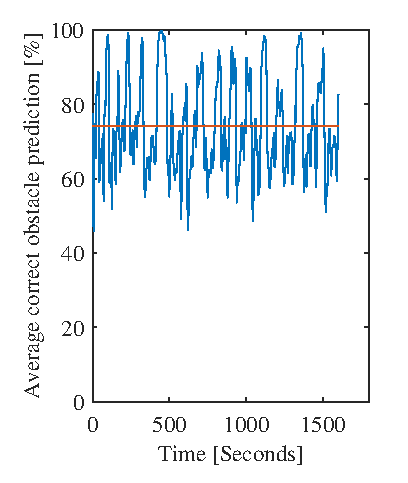
\includegraphics[width=1.0\textwidth]{chapters/mapping_of_dynamic_areas/figures/fremen_avg_miss_no_noise}	
        \caption{Prediction score without noise.}
        \label{fig:fremen_avg_miss_no_noise}
    \end{subfigure}
    \begin{subfigure}[t]{0.49\textwidth}
        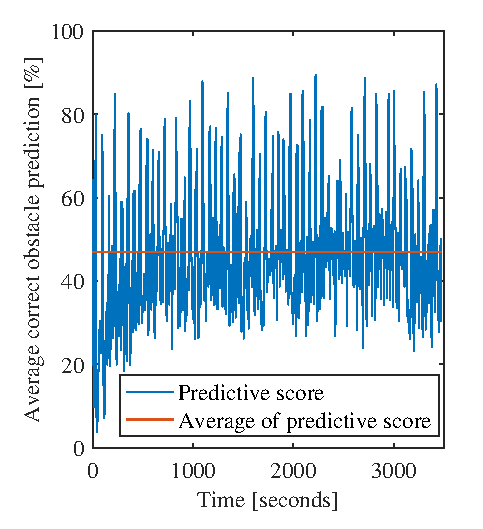
\includegraphics[width=1.0\textwidth]{chapters/mapping_of_dynamic_areas/figures/fremen_avg_miss_with_noise}
        \caption{Prediction score with noise.}
        \label{fig:fremen_avg_miss_with_noise}
    \end{subfigure}
    \caption{Prediction scores for FreMEn defined as the average number of matches between measured and predicted obstacles.}
    \label{fig:fremen_avg_correct_predictions}
\end{figure}

%!TEX root = ../../report.tex
\section{ Probabilistic Input  Markov Chain}
\label{sec:pmac}
The comparison between IMAC and HMM in figure \ref{fig:markow_learning} shows that incorporating the noise in the learning method has benefits. The HMM approaches the correct value as more observations are added. The HMM learning is slow at converging on a value, unlike IMAC. When there is no noise the IMAC 

\subsection{Developing on independent Markov chains}
The IMAC method considers an observation to be either occupied or free. In the system setup used in this project, however, the input is the probability that a cell is occupied. To use IMAC it is necessary to determine the state of the observation with one or two thresholds. The simplest choice is placing a threshold at $0.5$ rendering everything above as an occupied observation and everything below a free. This approach will make no distinction between an observation of $0.501$ and $0.999$, which both will be considered occupied and contribute equally in the learning process. This is not desirable as the latter measurement contains immensely more information than the former. 
Equating all measurements on the basis that they fall on the same side of a threshold reduces the advantage of taking position and sensor noise into consideration. An example could be a cell observed at a great distance and quite large uncertainty and then later very close by with high confidence in the reading. These two entries into the IMAC learner would carry the same weight. If for instance a reading resulted in a $0.99$ occupancy probability and a following reading produced a $0.49$ occupancy probability, the simple threshold method would register it as an occupied followed by a free and thus adding an event. In reality there is very little evidence for this event happening and if the subsequent reading would again produce a $0.99$ occupancy probability this would introduce even more dynamics disregarding that the evidence is very unsubstantiated. 

Therefore a method of incorporating the uncertainty of the observations and carrying them into the learner is desired. As IMAC is a fast learner of Markov transition probabilities when the observations are very certain, the incorporation of the uncertainties should not hinder that. 

The requirements for the incorporation of the uncertainties are:
\begin{itemize}
	\item Perform as IMAC on perfect input
	\item Avoid low confidence observations counting as much as high confidence
	\item Avoid biasing towards neither static or dynamic
\end{itemize}

The method devised to accomplish the integration of uncertainties is denoted probability input Markov chain (PMAC). As opposed to IMAC the PMAC uses a score rather than a count of a state and event. The state score is calculated as  \(2\cdot|0.5-p_{occ}|\) for the active state which is determined by whether \(p_{occ} > 0.5\) or not. This ensures that if the reading is certain, ie. either 0 or 1 the update will be similar to that of IMAC, and as uncertainty increases the score linearly decreases. The event score is calculated based on how certain the previous state was and how certain the current state is. In order to avoid biasing towards dynamic the maximum, based on the certainty of the previous state, is the average of the consecutive observations in that state. As the average cannot exceed 1 this ensures that in perfect certainty the behavior is equal to that of IMAC. The maximum limit based on the current state is the sum of scores in the current state.

\begin{equation}
IMAC: \lambda = \frac{\#event_{count}}{\#state_{obs}}
\end{equation}

\begin{equation}
PMAC: \lambda = \frac{\Sigma event_{score}}{\Sigma state_{score}}
\label{eq:pmac_lambda}
\end{equation}

\begin{equation}
state_{score}=2 \cdot |0.5-p_{occ}| 
\end{equation}

\begin{equation}
event_{score}=min(\hat{\mu}_{state_{score}}(i-1),state_{score}(i))
\end{equation}

Both the state and event scores behave as IMAC counters when the certainty is perfect, thus fulfilling the first requirement. The second requirement is achieved by the state score scaling with the occupancy probability distance from $0.5$, and the event score basing its value on the state score. Basing the state score on the distance from $0.5$ helps to avoid skewing the result towards static. Another possible scoring could be the probability for occupied and free respectively: 

\begin{equation}
score_{occ} = p_{occ}
\end{equation}
\begin{equation}
score_{free} = 1-p_{occ}
\end{equation}

As the active state is determined by a threshold of $0.5$, this scoring system would always be at least $0.5$, skewing the results. The chosen score better incorporates $0.5$ denoting unknown, thus producing a score of $0$. 

In order to avoid biasing towards dynamic the average of the previous state scores is used. If, instead, the sum had been used, a series of low confidence observations could skew the result. As the state score can be considered $\hat{\mu} \cdot n_{obs}$ the event score will be balanced when using as a maximum value. For instance $5$ observation with an occupancy probability of $0.6$ would each give a score of $0.2$, and the sum would consequently be $1$. Using the sum,  would be $1/1$  thus skewing it towards dynamics. Using the average, the event score is balanced to the state score and produces a more correct value of $0.2/1$. The correctness of this result is evident from the fact that simply counting events and states with IMAC also results in a probability on $\lambda = 1/5$. Hence the correct dynamics is estimated with PMAC and the parameters are only updated according to the confidence in the used observations.

\subsection{PMAC in action - an example}
Figure \ref{fig:state_scores_explained} shows an example of some observation, their occupied probabilities $p_{occ}$ and the subsequent state score. On the score plot the average of sequential observation in the same state are shown as green lines. This sets a maximum limit on the size of the subsequent event score. To demonstrate the workings of PMAC these observations are used as input to the PMAC learner in the following. 

\begin{figure} [htbp]
    \centering
    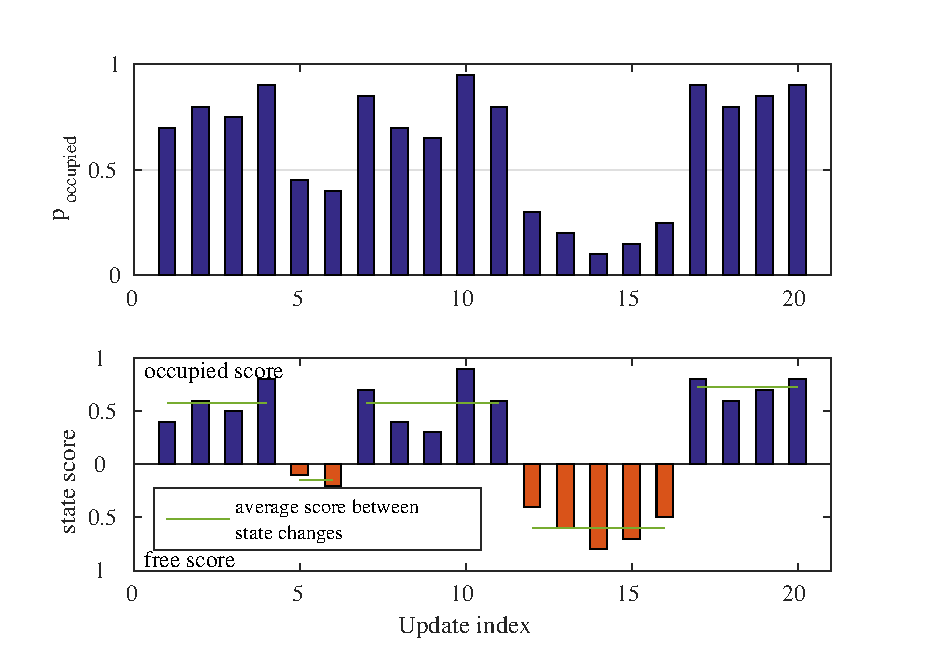
\includegraphics[scale=1]{chapters/mapping_of_dynamic_areas/figures/state_scores_explained}
    \caption{Artificial example of occupancy probabilities used to learn dynamics.}
    \label{fig:state_scores_explained}
\end{figure}

From the state scores in figure \ref{fig:state_scores_explained} it is seen that from index 0 to 11, the situation starts as occupied with quite confident readings. Then $2$ more uncertain reading showing free occurs before confident readings of occupied are again received. The effect of this on the exit is shown in figure \ref{fig:pmac_exit_explained}. The sum of occupied scores increases steadily from index $0$ to $11$, while the event sum increases a comparatively small amount. However it is clearly visible on the exit  value as it is the first observations and both sums are initialized to the smallest possible non-zero value. This initialization is chosen in order to avoid dividing by $0$ and minimizing the effect of the initialization on the result. The effects of this initialization is clearly visible in figure \ref{fig:pmac_entry_explained}, that shows the scores and values for the entry. The entry value is $1$, as the initial values causes, but as soon as input is received their effect is suppressed.

\begin{figure}[htbp]
\centering
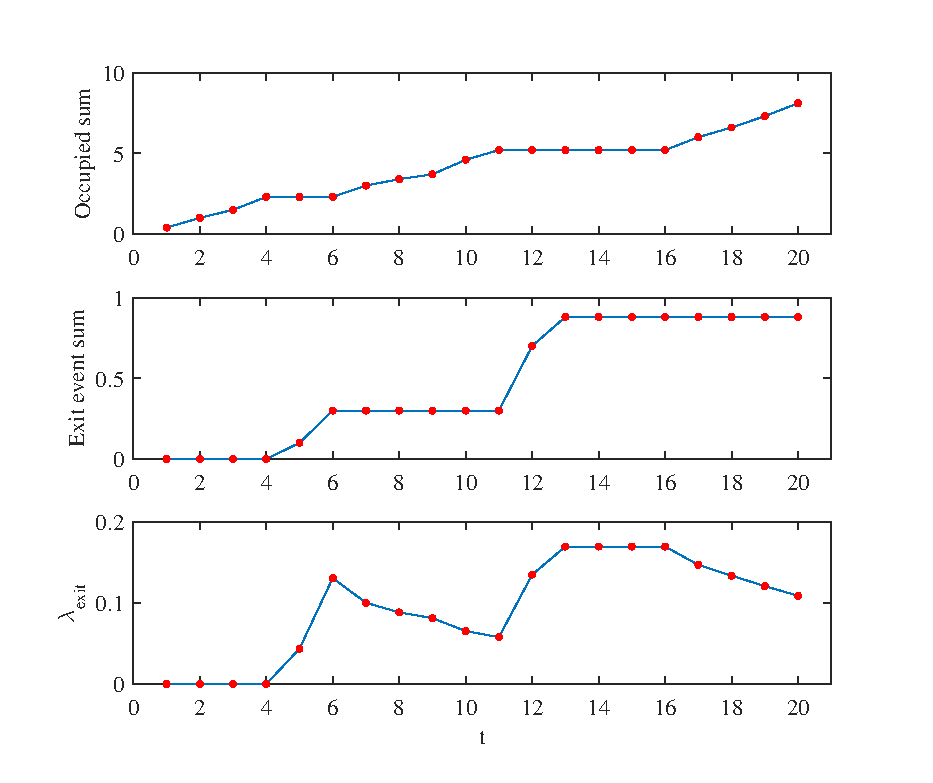
\includegraphics[scale=1]{chapters/mapping_of_dynamic_areas/figures/pmac_exit_explained}
\caption{Evolution of parameters used to estimate dynamics with the data shown in figure \ref{fig:state_scores_explained}.}
\label{fig:pmac_exit_explained}
\end{figure}

The observations from index $7$ to $20$ constitutes more certain changes in the state and thus carry more information which can be seen in the sums of especially the free score and entry event score. 

\begin{figure}[htbp]
    \centering
    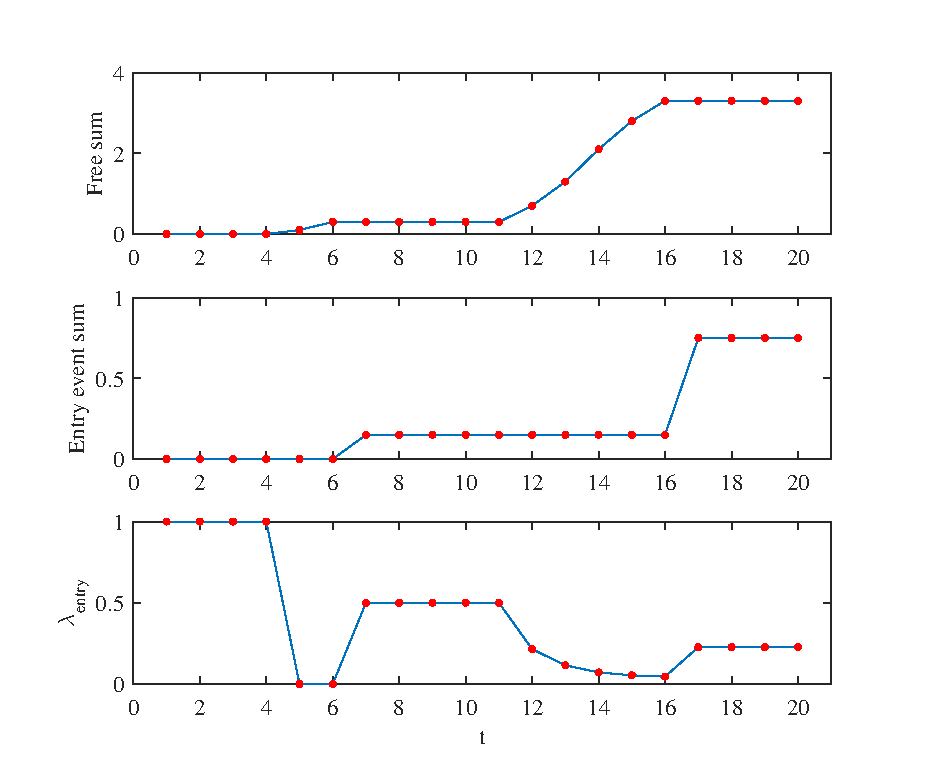
\includegraphics[scale=1]{chapters/mapping_of_dynamic_areas/figures/pmac_entry_explained}
    \caption{Evolution of parameters used to estimate dynamics with the data shown in figure \ref{fig:state_scores_explained}.}
    \label{fig:pmac_entry_explained}
\end{figure}

\todo{Write about improved pmac handling noise problem}

\begin{figure}[htbp]
\centering
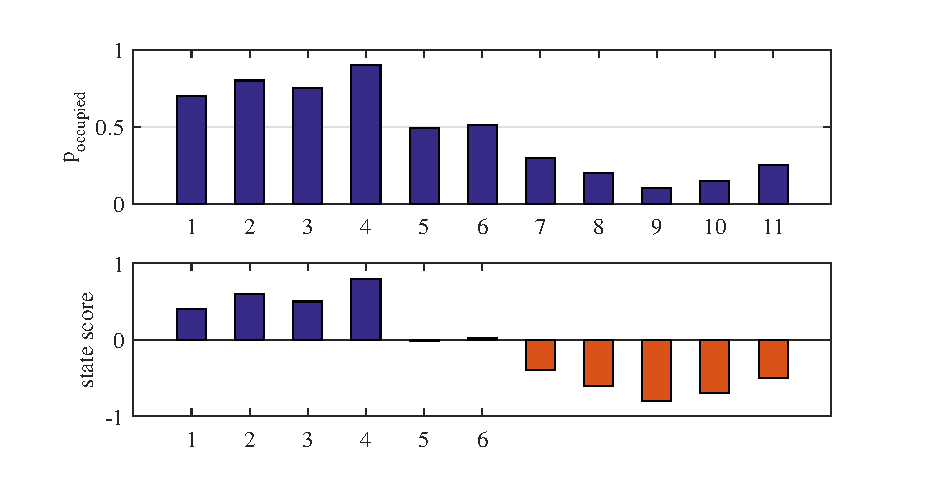
\includegraphics[scale=1]{chapters/mapping_of_dynamic_areas/figures/pmac_noise_problem_case}
\caption{}
\label{fig:pmac_noise_problem_case}
\end{figure}


\begin{figure}[htbp]
    \centering
    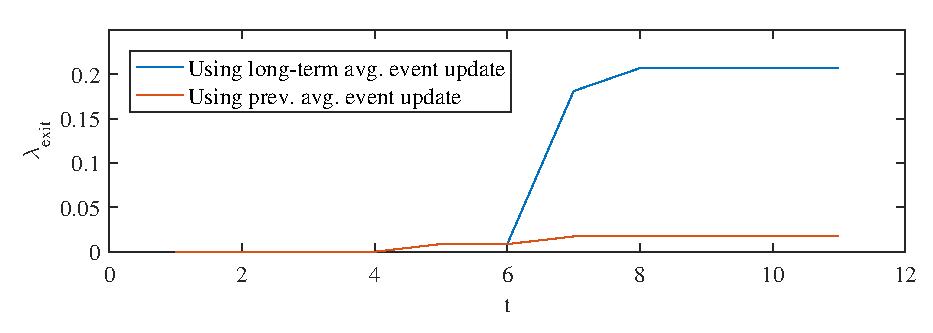
\includegraphics[scale=1]{chapters/mapping_of_dynamic_areas/figures/visualization_of_advantage_long_term_average}
    \caption{}
    \label{fig:visualization_of_advantage_long_term_average}
\end{figure}


\subsection{Comparing PMAC to alternavtives}
The goal of the developed PMAC learning method is to combine the fast learning under good condition from IMAC while also incorporating the uncertainty of sensor measurements. The uncertainty is represented as a probability from the static mapper that a cell is occupied. In order to compare PMAC to different Markov parameter learning methods, it has been tested in a simulation setup alongside IMAC and the online version of HMM. The test setup is one dimensional and a static mapper is used. The static mapper receives 10 noisy measurements, and determines the resulting occupied probability as learning input. The simulation is run for 200 learning rounds with the noise changing midway through. The initial noise is \(1.2\) grid cells then decreasing to \(0.11\) grid cells, both with zero mean. 

The result of simulation run is shown in figure \ref{fig:markow_learning_pmac_comparison_entry} and \ref{fig:markow_learning_pmac_comparison_exit}. Figure  \ref{fig:markow_learning_pmac_comparison_entry} shows the learning of the \(p_{entry}\) parameter. It is clear that all of the methods has difficulties learning the correct value. But after observation number 100, and the decrease in noise, both IMAC and PMAC increases towards the correct value, with PMAC catching up to IMAC. All the methods underestimate the \(p_{entry}\).

\begin{figure}[H]
	\centering
	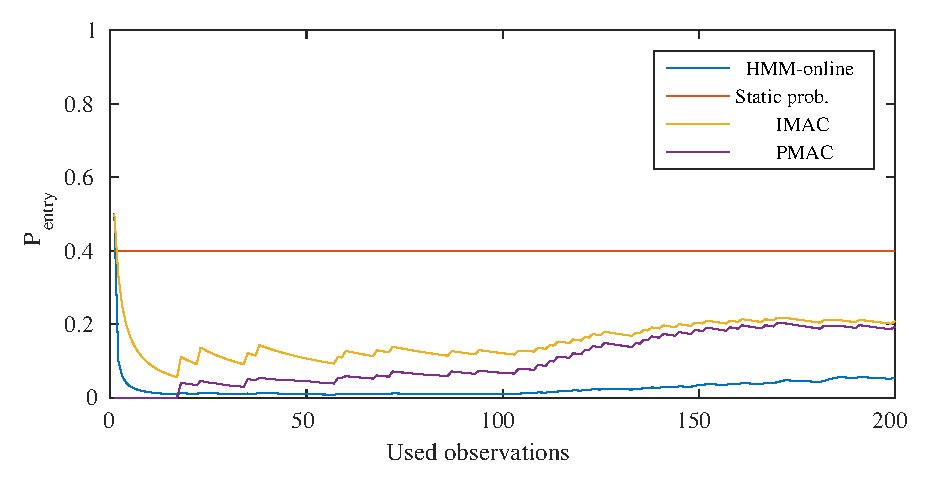
\includegraphics[scale=1]{chapters/mapping_of_dynamic_areas/figures/pmac_imac_hmm_entry}
	\caption{Estimated \(p_{entry}\) values for different learners}
	\label{fig:markow_learning_pmac_comparison_entry}
\end{figure}

The learning curves for \(p_{exit}\) is shown in figure \ref{fig:markow_learning_pmac_comparison_exit}. Contrary to the \(p_{entry}\) estimate the \(p_{exit}\) is overestimated, for the majority of the simulation. At observation number 100 it is seen that the decrease in noise has a significant effect on the estimates. PMAC experiences the most significant change when the noise changes. In the simulation shown the PMAC achieves the best result in estimating the \(p_{exit}\), but this is not consistently observed throughout all runs of the simulation. When the number of inputs, used in the static mapper before inputting to the learners, increases the difference between IMAC and PMAC becomes smaller as the static becomes increasingly certain on its output. 

\begin{figure}[H]
	\centering
	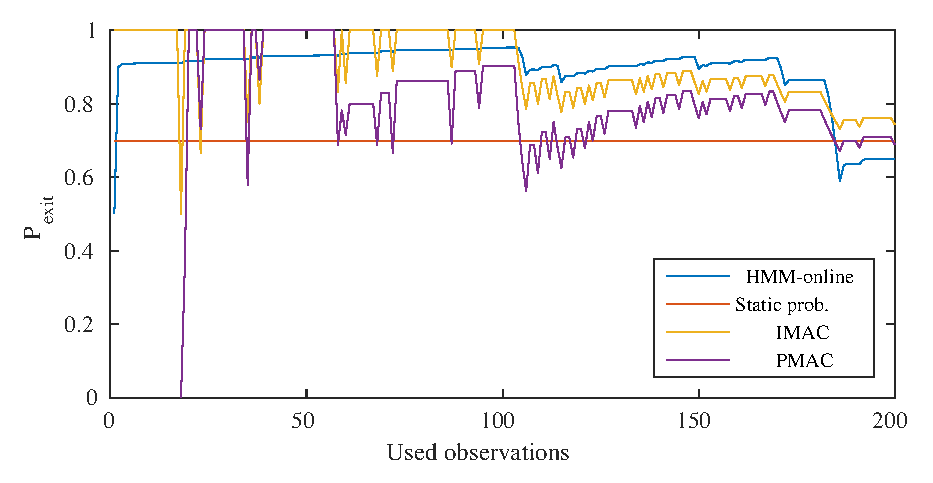
\includegraphics[scale=1]{chapters/mapping_of_dynamic_areas/figures/pmac_imac_hmm_exit}
	\caption{Estimated \(p_{exit}\) values for different learners}
	\label{fig:markow_learning_pmac_comparison_exit}
\end{figure}

The simulation shows that the ability of PMAC to learn the Markov parameters is at least comparable to the other learners when used with a static mapper, as intended. It is also observed that the static mapper increases the capabilities of IMAC to handle the zero-mean noise. The problem with IMAC, which were outline in [SECTION REFERENCE!!!!!!!!!!!!!], still remains which is why PMAC gains its credibility. 


\subsection{Initializing the dynamic map}
As the dynamic map is the result of a learning process it will not contain any information from the onset. 
This might be a problem if the localization and navigation systems are relying on the results to perform their tasks.
To handle this, but also to guide the dynamic map it is possible to initialize the PMAC parameters. 
This could be done by what has previously been learned by the PMAC or by a static map.
The initialization value of the PMAC parameters should be set according to the desired output, considering the interpretation, and  the confidence in the initial map.
If the confidence is high in the obstacles of the initializing map, giving the cells in the dynamic map a strong initialization helps ensure that small errors will have less effect. 
The same principles go for the free areas but it is likely might become obstructed at some point so initializing them too heavily might reduce the usefulness of the dynamic learner.
Three different types of initialization is available from a static map; free, occupied and unknown.
Each type can have different user-defined initialization values in order to accommodate various use-cases.  

%!TEX root = ../../report.tex
\section{Summary}


\begin{figure}[htbp]
	\centering
	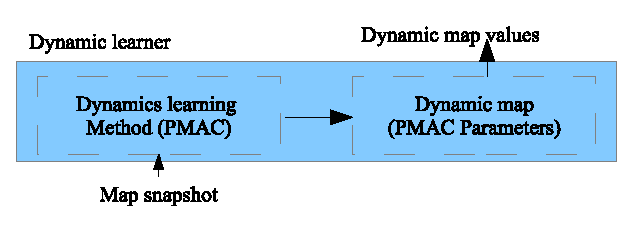
\includegraphics[scale=1]{chapters/mapping_of_dynamic_areas/figures/dynamic_detail.eps}
	\caption{The static mapping in the dynamic mapping system.}
	\label{fig:dynamic_learner_detail}
\end{figure}




%!TEX root = ../../report.tex
\chapter{Problem analysis}
\begin{figure}
	\centering
	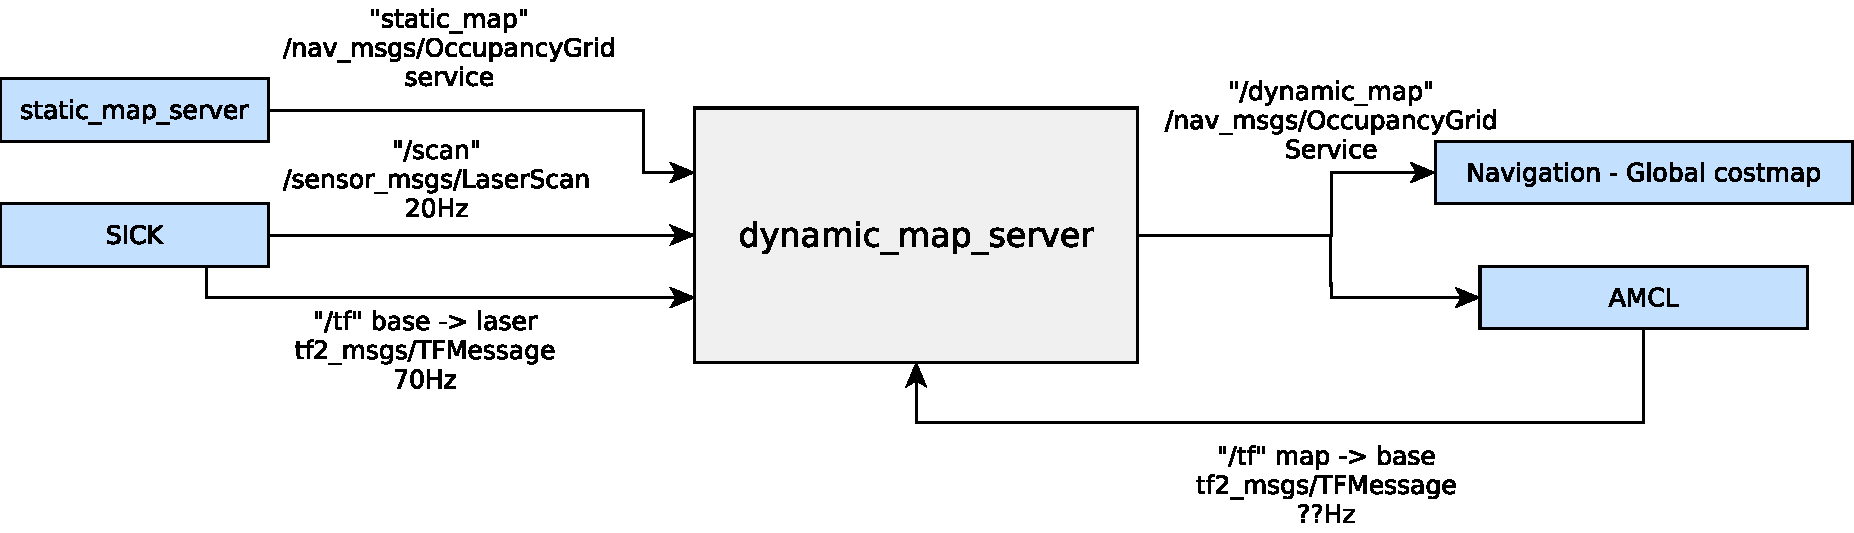
\includegraphics[width=0.6\linewidth]{figures/dynamic_map_mir_interface}
	\caption{Crossing point determined using P4P and an offset from the QR tag in its frame.}
	\label{fig:dyn_map}
\end{figure}
%!TEX root = ../../report.tex
\chapter{Evaluation}
%!TEX root = ../../report.tex
\chapter{Discussion and Conclusion}

Throughout this thesis a system was developed to handle the mapping, learning and representation of dynamic environments.
Specifically the aims of the thesis was:
\begin{enumerate}
	\item Precise mapping of static environments by incorporating sensor and localization noise
	\item Long-term, fast, adaptive map representation of dynamic environments
	\item Improved localization with a continuously adapted map of good features
	\item Integration and evaluation on the MiR-100 platform
\end{enumerate}

\section{Discussion}

 

\subsection{Precise Mapping of Static Environments by Incorporating Sensor and Localization Noise}
Tests and real world observations clearly showed the necessity of taking different noise sources into account. 
The developed method of incorporating noise was by a degradation of the update value for each observation. 
In order to account for the sensor noise the chosen sensor model is a reduced version of the ideal sensor model. 
This sensor model was chosen over the commonly used Elfes model due to its better evaluation scores. 
The Elfes model was developed to account for sensor noise but the localization noise present in the system overshadowed the effect of the sensor noise. 
The Elfes model was also tested with the same localization uncertainty weighting as the reduced ideal model and this improved the results of the Elfes model, but did not surpass the reduced ideal model. 
The simulation that the static mapping comparisons was based on might differ from real world experience due to differences in sensor noise and localization noise. 
The localization system used in the simulation is prior to version 1.5.1. of the MIR software. 
Version 1.5.1. introduced improvements to the localization system which may cause different results. 

\subsection{Long-term, Fast, Adaptive Map Representation of Dynamic Environments}
The representation of the dynamics in the environment is a Markov grid. 
Each cell contains an independent Markov process used to represent the probability that changes in state occur. 
The assumption that the process contained in each grid cell is independent is questionable. 
As most obstacles are larger than one cell it will cover multiple cells which will then enter and exit states together. 
Furthermore cells close to each other will probably have correlating states and changes due to the specific use of an area. 

In order to learn the parameters of the Markov processes the PMAC method was developed. 
This method was based on IMAC but with added incorporation of the static mapper, used in this project. 
The primary difference is the scores used to estimate the probability for a state being observed and a state change occurring.
As the Markov model operates with discrete states, and the Static mapper maps with continues occupancy probabilities, the scores are used to model the probability of a state. 
The probability for the cell being in a certain state now and a different state previously determines the probability for a state change.
The probability for a state change occurring must exist and the state and event scores are used to estimate this.  

The scores were developed to handle observations with widely varying certainty. 
In tests PMAC had mixed results. 
A difference in the accuracy of the two different transition probabilities was observed. 
The cause of the disparity might be an unbalance that stems from the sensor model. 
The sensor will clear multiple cells and only mark one. 
This is due to the model modelling the physical properties of a laser ray. 
The model found to be best at mapping static environments uses balanced values, the values of marking and clearing are equal but with opposite signs. 

\subsection{Improved Localization with a Continuously Adapted Map of Good Features}

In the evaluation test it was seen that the obstacles learned as static occupied helped increase the accuracy and precision of the localization compared to using an imperfect static map. 

A threat to the continued reliability of the dynamic mapping is the possible feedback from bad localization estimates. 
If the localization is consistently wrong in an area the features learned might be offset which could cause further degradation of the pose estimate.
This scenario will partly violate an assumption in the dynamic mapping system. 
It is assumed that the world changes slowly enough to provide reasonably accurate pose estimates until an updated map is provided. 
If the robot only rarely observes areas slower changes might over time cause enough discrepancy between the map and the environment to cause localization failure.
In such cases a full SLAM solution is required.
In industrial settings it is likely that a robot operates along fixed routes or within certain areas. This means that that area of operation will be frequently visited and thus reduce the risk of these failures.

Even if a local area has not been closely mapped for some time, if it is within sight areas where updated maps are available this can improve the localization. 
This was seen in the localization test where better localization was achieved by using the learned map, even though the map was learned under imprecise localization.

\section{Conclusion}
\section{Future Work}

The static mapper currently incorporates the various noise by reducing the update values in the map. 
A possible improvement to the weighting could be considering the entire covariance matrix instead of the individual standard deviation. 
Using the noise more proactive could also improve the mapping results and should help converging faster towards the correct result.
Seen as the localization noise is a significant influence on the mapping any improvement in the accuracy would also benefit the mapping.


The learner showed unbalanced learning of the two transition probabilities.
It is believed that the origins of these problems stems from the static mapping. 
A mapping method that more accurately incorporates the noise could help solve this challenge. 


The classification for converting the dynamics into maps for the localization was handled by a manually designed classifier.
By obtaining vast amounts of data it might be possible to improve the classification through machine learning techniques. 


To continue the development of the Dynamic mapping system it would be beneficial to evaluate the long term performance of the system. 
This should investigate the long-term effects of the feedback between the localization and the dynamic mapping.



\subsection{future notes}

Precise mapping of static environment by incorporation of sensor and localization noise
Separation of sensor and localisation noise?
Used aktively instead of just towards unknown?
Use of feedback from further on, maybe a blueprint map
Brug principle component scores af covariance istedet for bare summen af std afvigelser i reduced ideal inverse sensor model. Det andet underestimate ved kun at se på projektionerne ind i akserne. Muligvis kan determinanten(arealet i en standard afvigelses konfidens elipse.)
Korrekt Indkorporering af sensorstøj burde resultere i hurtigere convergering mod korrekt kort. Sådan en burde laves.
2. Long-term fast adaptive map representation of dynamic environments

3. Improved localization with a continuously adapted map of good features
The classification
More data -> better classification
Machine learning techniques?

A better use (future work)
Localization -> use more values
Planner -> balancing the the cost


4. Integration and evaluation on the MiR-100 platform
Evaluation methods
Evaluation only for hours, but a large scale evaluation in industrial for weeks is required to show long term adaptation to changes and learning real obstacles dynamic



\pagebreak
\pagenumbering{roman}
\appendix
\appendixpage
%!TEX root = ../../report.tex
\chapter{Appendix}
The estimated $\lambda$ values are shown in figure \ref{fig:all_learnings_sim_1} and \ref{fig:all_learnings_sim_2}. The estimated values in the plots are calculated by the average estimate in an area around the obstacles. The requirement for a cell to be used in the average was all parameters, the state and event scores, were above 0.5. As this method deviates from the scoring method used for comparison the result are not directly comparable.
The figures gives an overview of the speed of leaning but as many cells are included that might mainly learn based on noise is may not represent an accurate image of the learning accuracy.


\begin{figure}[htbp]
	\begin{subfigure}[t]{0.5\linewidth}
		\centering
		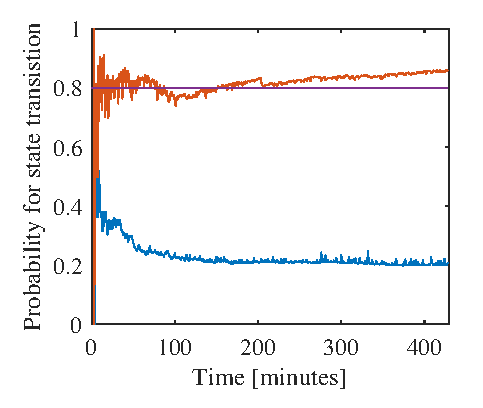
\includegraphics[width=1\linewidth]{chapters/appendix/figures/learning_curves/obs1}
		\caption{1}
	\end{subfigure}
	\hspace*{\fill}
	\begin{subfigure}[t]{0.5\linewidth}
		\centering
		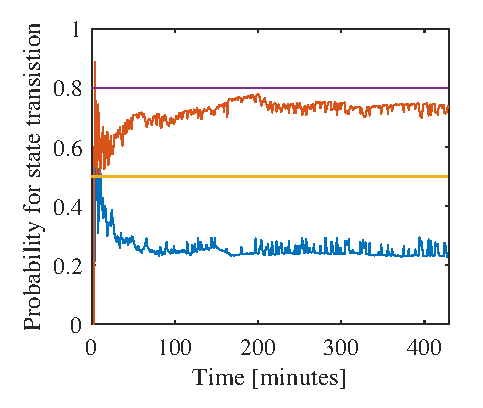
\includegraphics[width=1\linewidth]{chapters/appendix/figures/learning_curves/obs2}
		\caption{2}
	\end{subfigure}


	\begin{subfigure}[t]{0.5\linewidth}
		\centering
		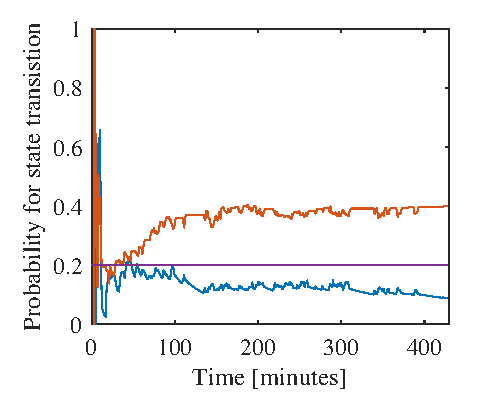
\includegraphics[width=1\linewidth]{chapters/appendix/figures/learning_curves/obs3}
		\caption{3}
	\end{subfigure}
	\hspace*{\fill}
	\begin{subfigure}[t]{0.5\linewidth}
		\centering
		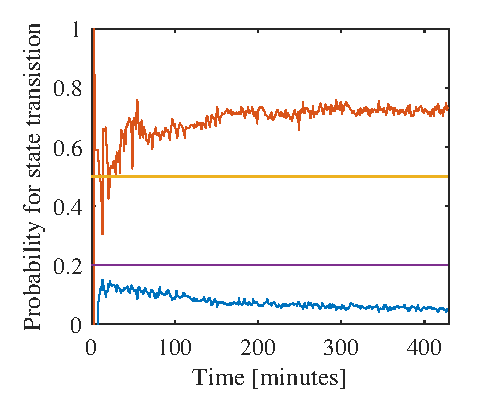
\includegraphics[width=1\linewidth]{chapters/appendix/figures/learning_curves/obs4}
		\caption{4}
	\end{subfigure}
	
	\hspace*{\fill}
	\begin{subfigure}[t]{0.5\linewidth}
		\centering
		
\includegraphics[scale = 1]{chapters/appendix/figures/learning_curves/legend}
		\caption{1}
	\end{subfigure}
	\hspace*{\fill}

	\caption{CAPTION}
	\label{fig:all_learnings_sim_1}
\end{figure}

\begin{figure}[htbp]
	\begin{subfigure}[t]{0.5\linewidth}
		\centering
		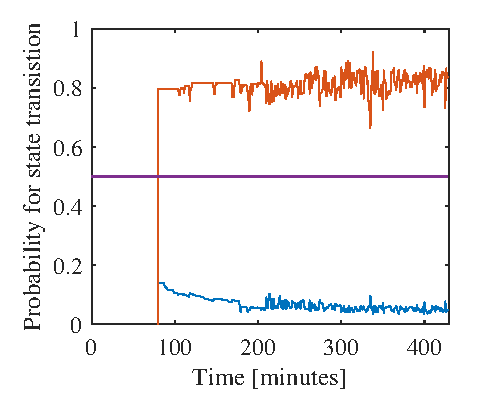
\includegraphics[width=1\linewidth]{chapters/appendix/figures/learning_curves/obs5}
		\caption{5}
	\end{subfigure}
	\hspace*{\fill}
	\begin{subfigure}[t]{0.5\linewidth}
		\centering
		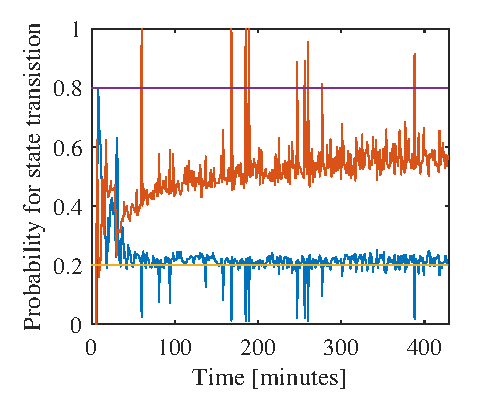
\includegraphics[width=1\linewidth]{chapters/appendix/figures/learning_curves/obs6}
		\caption{6}
	\end{subfigure}
	
	\begin{subfigure}[t]{0.5\linewidth}
		\centering
		\includegraphics[width=1\linewidth]{chapters/appendix/figures/learning_curves/obs7}
		\caption{7}
	\end{subfigure}
	\hspace*{\fill}
	\begin{subfigure}[t]{0.5\linewidth}
		\centering
		\includegraphics[width=1\linewidth]{chapters/appendix/figures/learning_curves/obs8}
		\caption{8}
	\end{subfigure}


	\begin{subfigure}[t]{0.5\linewidth}
		\centering
		\includegraphics[width=1\linewidth]{chapters/appendix/figures/learning_curves/obs9}
		\caption{9}
	\end{subfigure}
	\hspace*{\fill}
	\begin{subfigure}[t]{0.5\linewidth}
		\centering
		\includegraphics[scale = 1]{chapters/appendix/figures/learning_curves/legend}
		\caption{1}
	\end{subfigure}

	\caption{CAPTION}
	\label{fig:all_learnings_sim_2}
\end{figure}

\backmatter
\printbibliography[heading=bibintoc]

\end{document}